\documentclass[11pt,a4paper]{article}

% Inclusión de configuración y paquetes
% ==============================================================================
% Paquetes base y codificación
% ==============================================================================
\usepackage[utf8]{inputenc}
\usepackage[T1]{fontenc}
\usepackage[spanish, es-tabla, es-nodecimaldot]{babel}
\usepackage{csquotes}

% Márgenes formato APA 7 (1 pulgada / 2.54 cm en todos los lados)
\usepackage[margin=2.54cm, headheight=16pt]{geometry}

% Tipografía clásica y espacio interlineal (APA 7 estándar: 1.5)
\usepackage{mathptmx}
\usepackage{setspace}
\onehalfspacing

% Paquetes matemáticos rigurosos
\usepackage{amsmath}
\usepackage{amssymb}
\usepackage{amsfonts}
\usepackage{mathtools}

% Figuras y tablas profesionales bajo estándar APA 7 (sin líneas verticales)
\usepackage{graphicx}
\graphicspath{{./}{figuras/}{./figuras/}}
\usepackage{float}
\usepackage{booktabs}
\usepackage{tabularx}
\usepackage{etoolbox}
\usepackage{multirow}
\usepackage{makecell}
\usepackage{array}
\AtBeginEnvironment{table}{\fontsize{10}{12.5}\selectfont\centering}
\usepackage{caption}
\usepackage{subcaption}

% Formato de títulos de figuras y tablas según APA 7
\DeclareCaptionLabelSeparator{newline}{\newline}
\captionsetup[figure]{
    labelfont=bf,
    textfont=it,
    labelsep=newline,
    singlelinecheck=false,
    justification=raggedright
}
\captionsetup[table]{
    labelfont=bf,
    textfont=it,
    labelsep=newline,
    singlelinecheck=false,
    justification=raggedright
}

% Diagramas vectoriales con TikZ
\usepackage{tikz}
\usetikzlibrary{arrows.meta, positioning, shapes.geometric, backgrounds, babel}

% Encabezados y numeración formal
\usepackage{fancyhdr}
\pagestyle{fancy}
\fancyhf{}
\fancyhead[L]{\small\itshape Universidad Nacional de San Antonio Abad del Cusco}
\fancyhead[R]{\small\thepage}
\renewcommand{\headrulewidth}{0.4pt}
\renewcommand{\footrulewidth}{0pt}

% Enlaces y URLs con corte automático de línea
\usepackage{xurl}
\usepackage{xcolor}
\usepackage{hyperref}
\hypersetup{
    colorlinks=true,
    breaklinks=true,
    linkcolor=blue!80!black,
    citecolor=blue!80!black,
    urlcolor=blue!80!black,
    pdftitle={Rutas Mínimas con Distintas Colas de Prioridad en Redes Viales Urbanas de la Ciudad del Cusco},
    pdfauthor={Grupo 5 - UNSAAC}
}

% Ajustes microtipográficos para evitar Overfull hbox
\usepackage{microtype}
\emergencystretch=2.5em
\tolerance=2000
\hbadness=2000

% Sangría de primera línea estilo APA
\setlength{\parindent}{1.27cm}
\setlength{\parskip}{0.3em}

% Citas y Referencias - Estilo APA 7ma Edición (BibLaTeX + Biber)
\usepackage[
    backend=biber,
    style=apa,
    sorting=nyt
]{biblatex}
\DeclareLanguageMapping{spanish}{spanish-apa}
\addbibresource{referencias.bib}

% Algoritmos y pseudocódigo
\usepackage{algorithm}
\usepackage{algorithmic}

% Inclusión de código fuente (Python)
\usepackage{listings}
% ==============================================================================
% Configuración de listings para inserción de código Python con soporte UTF-8
% ==============================================================================
\definecolor{codegreen}{rgb}{0,0.6,0}
\definecolor{codegray}{rgb}{0.5,0.5,0.5}
\definecolor{codepurple}{rgb}{0.58,0,0.82}
\definecolor{backcolour}{rgb}{0.96,0.97,0.98}

\lstdefinestyle{pythonstyle}{
    backgroundcolor=\color{backcolour},
    commentstyle=\color{codegreen}\itshape,
    keywordstyle=\color{blue}\bfseries,
    numberstyle=\fontsize{7}{9}\selectfont\color{codegray},
    stringstyle=\color{codepurple},
    basicstyle=\ttfamily\fontsize{8}{10.5}\selectfont,
    breakatwhitespace=false,
    breaklines=true,
    captionpos=b,
    keepspaces=true,
    numbers=left,
    numbersep=6pt,
    xleftmargin=12pt,
    aboveskip=0.8em,
    belowskip=0.8em,
    showspaces=false,
    showstringspaces=false,
    showtabs=false,
    tabsize=4,
    frame=single,
    framesep=4pt,
    rulecolor=\color{black!20},
    inputencoding=utf8,
    extendedchars=true,
    literate=
      {á}{{\'a}}1 {é}{{\'e}}1 {í}{{\'i}}1 {ó}{{\'o}}1 {ú}{{\'u}}1
      {Á}{{\'A}}1 {É}{{\'E}}1 {Í}{{\'I}}1 {Ó}{{\'O}}1 {Ú}{{\'U}}1
      {ñ}{{\~n}}1 {Ñ}{{\~N}}1
}

\lstset{style=pythonstyle}



\begin{document}

% =========================================================================
% PORTADA INSTITUCIONAL - UNSAAC (GRUPO 5)
% =========================================================================
\begin{titlepage}
    \centering
    \vspace*{-0.5cm}
    
    {\fontsize{13}{16}\selectfont \textbf{UNIVERSIDAD NACIONAL DE SAN ANTONIO ABAD DEL CUSCO}}\\[0.25cm]
    {\fontsize{11}{14}\selectfont \textbf{FACULTAD DE INGENIERÍA ELÉCTRICA,}}\\
    {\fontsize{11}{14}\selectfont \textbf{ELECTRÓNICA, INFORMÁTICA Y MECÁNICA}}\\[0.25cm]
    {\fontsize{11}{14}\selectfont \textbf{ESCUELA PROFESIONAL DE INGENIERÍA INFORMÁTICA}}\\
    {\fontsize{11}{14}\selectfont \textbf{Y DE SISTEMAS}}\\[0.6cm]
    
    
\includegraphics[width=3.8cm]{figuras/escudo.png}\\[0.5cm]
    
    {\fontsize{13}{16}\selectfont \textbf{INFORME TÉCNICO DE INVESTIGACIÓN FORMATIVA}}\\[0.3cm]
    \rule{\textwidth}{1.2pt}\\[0.35cm]
    {\fontsize{13}{16.5}\selectfont \textbf{“RUTAS MÍNIMAS CON DISTINTAS COLAS DE PRIORIDAD EN REDES VIALES URBANAS DE LA CIUDAD DEL CUSCO”}}\\[0.25cm]
    \rule{\textwidth}{1.2pt}\\[0.6cm]
    
    \begin{minipage}{0.88\textwidth}
        \setstretch{1.2}
        \textbf{Asignatura:} ALGORITMOS AVANZADOS (Semestre 2026-2)\\[0.25cm]
        \textbf{Docente Responsable:} Ing. Héctor Eduardo Ugarte Rojas\\[0.25cm]
        \textbf{Identificador:} GRUPO 5\\[0.25cm]
        \textbf{Integrantes:}\\[0.2cm]
        \begin{tabularx}{\linewidth}{@{}Xr@{}}
          \textbullet\quad Choquenaira Quispe, Noe Franklin & 133962\\[0.15cm]
          \textbullet\quad Porroa Sivana, Yeni Ruth & 120893\\[0.15cm]
          \textbullet\quad Quispe Rimachi, Romario & 164257\\[0.15cm]
          \textbullet\quad Yaranga Achahui, Aldo & 103179
        \end{tabularx}
    \end{minipage}\\[0.4cm]
    
    \vfill
    {\textbf{Cusco – Perú – 2026}}\\[0.2cm]
\end{titlepage}

% =========================================================================
% SECCIONES PRELIMINARES: RESUMEN Y ABSTRACT (NÚMEROS ROMANOS)
% =========================================================================
\pagenumbering{roman}
\setcounter{tocdepth}{3}
\setcounter{secnumdepth}{3}

% Resumen y Abstract (aparecen en el índice como secciones preliminares)
\section{Resumen}

Este proyecto compara tres colas de prioridad dentro del mismo algoritmo de Dijkstra para resolver el problema de caminos mínimos desde un origen único en redes viales urbanas: un min-heap binario indexado, un heap 4-ario indexado y un Fibonacci heap. El caso aplicado utiliza una consulta sobre una red vial real de Cusco obtenida de OpenStreetMap (891 vértices y 2139 aristas dirigidas), mientras que la comparación controlada se realiza sobre instancias sintéticas reproducibles con perfiles disperso ($|E|=4|V|$) y denso ($|E|=0.08\,|V|(|V|-1)$). El protocolo mide tiempo con \texttt{perf\_counter\_ns}, desactiva el recolector de basura durante cada muestra, ejecuta 15 repeticiones sobre tres instancias por escala y reporta mediana e intervalo intercuartílico; la corrección se valida contra NetworkX y un certificado de Bellman que verifica también que cada cadena de predecesores llegue al origen. Sin caminos materializados cuesta $O(|V|+|E|)$; comprobar los caminos explícitos requiere además leer su longitud total.

Los resultados no permiten declarar una cola ganadora universal. El heap 4-ario obtiene la menor mediana en 7 de 10 escalas sintéticas, con una razón mediana de 0.96 frente al heap binario en el perfil disperso y 0.95 en el denso, pero los intervalos intercuartílicos se solapan en las 10 escalas y el heap binario gana en 3 escalas y en la consulta OSM (15.65 ms frente a 19.87 ms del 4-ario y 26.09 ms del Fibonacci). El Fibonacci heap nunca obtiene la menor mediana y resulta entre 1.05 y 1.59 veces más lento que el binario. La extensión $A^*$ reduce las expansiones de 887 a 823 ($-7.2\%$) sin alterar el costo óptimo. Un factor meteorológico uniforme de 1.0691 incrementa el tiempo estimado en $6.91\%$, pero no modifica la ruta porque escala todos los pesos por igual. La conclusión central es que la elección de cola depende de la escala, la densidad y el entorno de ejecución, y que la ventaja asintótica del Fibonacci heap no se traduce en ventaja práctica en esta implementación de Python.

\vspace{0.4cm}
\noindent\textbf{Palabras clave:} algoritmo de Dijkstra, colas de prioridad, heap binario, heap 4-ario, Fibonacci heap, rutas mínimas, OpenStreetMap, Cusco, $A^*$, análisis experimental.

\newpage

\vspace{0.8cm}
\section*{Abstract}
\addcontentsline{toc}{section}{Abstract}

This project evaluates three priority queues within the same Dijkstra implementation for the single-source shortest-path problem on urban road networks: an indexed binary min-heap, an indexed 4-ary heap, and a Fibonacci heap. The applied case uses a real Cusco road network retrieved from OpenStreetMap, with 891 vertices and 2139 directed edges. The controlled comparison uses reproducible sparse ($|E|=4|V|$) and dense ($|E|=0.08\,|V|(|V|-1)$) synthetic instances. The protocol records wall-clock time with \texttt{perf\_counter\_ns}, disables garbage collection during each sample, executes 15 repetitions on three instances per scale, and reports medians and interquartile ranges. Correctness is checked against NetworkX and a Bellman certificate that also verifies that every predecessor chain reaches the source. Computing distances without materialized paths takes $O(|V|+|E|)$; validating explicit paths additionally reads their total length.

The results do not support a universal winner. The 4-ary heap obtains the lowest median in 7 of 10 synthetic scales, with median ratios of 0.964 relative to the binary heap in the sparse profile and 0.954 in the dense profile. However, the interquartile ranges overlap at every scale. The binary heap wins in the remaining 3 scales and in the OSM query, where its median is 15.65 ms, compared with 19.87 ms for the 4-ary heap and 26.09 ms for the Fibonacci heap. The Fibonacci heap never obtains the lowest median and is between 1.05 and 1.59 times slower than the binary heap. The $A^*$ extension reduces expansions from 887 to 823 ($-7.2\%$) without changing the optimal cost. A uniform weather factor of 1.0691 increases the estimated time by $6.91\%$ without changing the route because it scales all weights equally. These findings indicate that queue selection depends on scale, graph density, and runtime environment; the asymptotic advantage of the Fibonacci heap does not translate into a practical advantage in this Python implementation.

\vspace{0.4cm}
\noindent\textbf{Keywords:} Dijkstra's algorithm, priority queues, binary heap, 4-ary heap, Fibonacci heap, shortest paths, OpenStreetMap, Cusco, $A^*$, experimental analysis.

\newpage

\begingroup
\hypersetup{linkcolor=black}
\color{black}
\setstretch{1.10}
\setlength{\parskip}{1pt}
\fontsize{10}{12.5}\selectfont
\tableofcontents
\newpage

\listoffigures
\vspace{0.6cm}
\listoftables
\endgroup
\hypersetup{linkcolor=blue!80!black}
\newpage

% =========================================================================
% CUERPO PRINCIPAL DEL INFORME (INICIA EN 1 CON INTRODUCCIÓN)
% =========================================================================
\pagenumbering{arabic}
\setcounter{section}{0}

% Sección 1: Introducción
\section{Introducción}
\label{sec:introduccion}

\subsection{Contexto y Motivación}
La determinación eficiente de rutas mínimas en redes viales urbanas representa uno de los problemas fundamentales y de mayor impacto práctico en la ciencia de la computación, la ingeniería de transporte y la logística de atención a emergencias. En entornos metropolitanos contemporáneos, los sistemas de despacho para ambulancias, unidades de bomberos y patrullaje policial requieren calcular trayectorias óptimas en fracciones de segundo para minimizar los tiempos de respuesta, donde reducciones marginales de tiempo se traducen directamente en la preservación de vidas humanas.

La ciudad del Cusco, ubicada en la sierra sur del Perú a una altitud media de 3,399 m s. n. m., presenta una morfología urbana singular. Su Centro Histórico, declarado Patrimonio de la Humanidad por la UNESCO en 1983, superpone una traza urbana incaica y colonial caracterizada por calzadas sumamente angostas, pasajes adoquinados, alta densidad de giros obligatorios y severas pendientes topográficas que oscilan con frecuencia entre el 5\% y más del 15\%. En este contexto geográfico, la distancia euclidiana o la longitud puramente física de un tramo vial resultan insuficientes como métrica de optimización. Un trayecto físicamente más corto pero con un gradiente positivo pronunciado impone un esfuerzo motriz severo sobre un vehículo pesado de emergencia, reduciendo drásticamente su velocidad operativa y aumentando el riesgo de demoras críticas. Por ende, resulta imperativo formular modelos de costo generalizado que integren la topografía andina y evaluar algoritmos de caminos mínimos capaces de procesar mallas viales a gran escala con alta eficiencia temporal y espacial.

\subsection{Planteamiento del Problema}
El Algoritmo de Dijkstra \parencite{dijkstra1959note} es el estándar canónico para resolver el problema de caminos mínimos desde un origen único (\textit{Single-Source Shortest Path}, SSSP) en grafos dirigidos con pesos no negativos ($w(e) \ge 0$). La complejidad asintótica de este algoritmo depende intrínsecamente de la estructura de datos utilizada para implementar la cola de prioridad que gestiona los vértices tentativos:
\begin{equation}
    T(|V|, |E|) = O(|V| \cdot T_{\text{Extract-Min}} + |E| \cdot T_{\text{Decrease-Key}} + |V| \cdot T_{\text{Insert}})
\end{equation}

En la literatura teórica clásica, el Fibonacci Heap propuesto por \textcite{fredman1987fibonacci} ostenta la cota asintótica óptima conocida de $O(|E| + |V| \log |V|)$, al ejecutar la operación de disminución de clave (\texttt{Decrease-Key}) en tiempo amortizado $O(1)$ y la extracción del mínimo (\texttt{Extract-Min}) en $O(\log |V|)$. No obstante, estudios computacionales de referencia \parencite{cherkassky1996shortest,lamarca1996cache} han reportado que, en redes dispersas donde $|E| = O(|V|)$ (como las redes viales donde el grado promedio por nodo rara vez supera 4), la constante oculta en la notación asintótica del Fibonacci Heap, originada por la alocación dinámica en memoria, la manipulación de múltiples punteros y los fallos en las líneas de caché (\textit{cache misses}), degrada su rendimiento en tiempo real frente a montículos contiguos como el Binary Heap o el $d$-ary Heap.

El problema central que aborda este proyecto radica en investigar, implementar y contrastar cuantitativamente el comportamiento empírico y teórico de distintas colas de prioridad acopladas al algoritmo de Dijkstra, evaluando su desempeño real sobre la red vial urbana del Cusco bajo una función de costo generalizado con impedancia topográfica.

\subsection{Objetivos del Proyecto}

\subsubsection{Objetivo General}
Diseñar, implementar y evaluar experimentalmente una solución computacional modular para el cálculo de rutas mínimas en la red vial urbana de la ciudad del Cusco, contrastando el desempeño en tiempo de ejecución, operaciones elementales y consumo de memoria del Algoritmo de Dijkstra instrumentado con tres estructuras de colas de prioridad: Min-Heap Binario Indexado, $d$-ary Heap y Fibonacci Heap, verificando formalmente la optimalidad de las soluciones.

\subsubsection{Objetivos Específicos}
Siguiendo la metodología de ingeniería de software y análisis de algoritmos, los objetivos específicos se ordenan en cuatro fases secuenciales e integradas:
\begin{enumerate}
    \item \textbf{OE1 (Modelar):} Formular el modelo matemático del grafo vial dirigido del Centro Histórico del Cusco y su extensión a la red metropolitana OpenStreetMap, definiendo una función de costo generalizado (impedancia andina) que cuantifique el impacto de calles de un solo sentido, calles angostas coloniales, pasajes peatonales y gradientes altitudinales positivos.
    \item \textbf{OE2 (Diseñar e Implementar):} Diseñar e implementar bajo una arquitectura desacoplada en cuatro capas lógicas el algoritmo de Dijkstra parametrizado, integrando tres alternativas de colas de prioridad puras con soporte formal para \texttt{Decrease-Key}: Min-Heap Binario Indexado, 4-ary Heap ($d=4$) optimizado para líneas de caché L1/L2, y Fibonacci Heap amortizado, extendiendo el sistema hacia búsqueda heurística $A^*$.
    \item \textbf{OE3 (Verificar):} Validar analíticamente la correctitud del algoritmo mediante traza manual paso a paso, certificado formal de optimalidad independiente en $O(|V|+|E|)$ y una suite automatizada de pruebas unitarias bajo el patrón Arrange-Act-Assert (AAA), contrastando los resultados contra oráculos canónicos de referencia (NetworkX y Bellman-Ford).
    \item \textbf{OE4 (Evaluar e Investigar):} Evaluar experimentalmente la escalabilidad asintótica, el consumo de operaciones elementales y los tiempos de CPU en redes viales sintéticas controladas y en la red vial real OSM de Cusco, contrastando la teoría asintótica clásica frente a la localidad espacial de memoria caché en hardware contemporáneo.
\end{enumerate}

\subsection{Alcance y Delimitación}
El proyecto se delimita formalmente en las siguientes dimensiones:
\begin{itemize}
    \item \textbf{Delimitación Espacial:} Se analizan dos escalas complementarias: (1) La malla vial nuclear del Centro Histórico del Cusco (6 intersecciones estratégicas: Plaza Mayor, Plaza Regocijo, Qorikancha, Plaza San Francisco, Mercado Central San Pedro y Plazoleta Limacpampa), empleada para traza manual analítica y verificación paso a paso; y (2) La red vial urbana real de Cusco extraída de OpenStreetMap vía OSMnx \parencite{boeing2017osmnx}, con un radio de 1,500 m, 891 vértices y 2,139 aristas dirigidas.
    \item \textbf{Delimitación Algorítmica:} Se evalúa el algoritmo de Dijkstra en grafos dirigidos estáticos con costos deterministas no negativos ($w(e) \ge 0$). Como extensión de ruteo punto a punto se integra $A^*$ con heurística consistente. Bellman-Ford y NetworkX operan exclusivamente como oráculos independientes de verificación cruzada.
    \item \textbf{Alcance del Sistema:} Comprende la formulación matemática integral, la solución analítica manual, el núcleo ejecutable en Python 3.12 con interfaz de línea de comandos (CLI), la aplicación interactiva web en Streamlit, el cuaderno didáctico en Google Colab y la suite automatizada de 278 pruebas con Pytest.
\end{itemize}

\subsection{Control de Versiones y Repositorio Oficial en GitHub}
Conforme a las directrices de reproducibilidad y trabajo colaborativo del curso, el desarrollo íntegro del proyecto se gestiona bajo el sistema de control de versiones Git y se aloja en el repositorio público oficial:
\begin{center}
    \url{https://github.com/frankich99/PROYECTO_Algoritmos-Avanzados-UNSAAC}
\end{center}
La organización de ramas adopta un esquema estructurado: la rama \texttt{main} almacena las versiones estables consolidadas, complementada por ramas de desarrollo temáticas por integrante (\texttt{ramaFRANKI}, \texttt{ramaAldo}, \texttt{ramaYeni}, \texttt{RamaRomario}). Los datos experimentales se versionan en \texttt{python/data/processed/} para garantizar reproducibilidad total sin requerir descargas en vivo de APIs externas.

\subsection{Organización del Documento}
El presente informe técnico se organiza conforme a los requerimientos temáticos del apartado 9 del sílabo:
La Sección~\ref{sec:introduccion} presenta la introducción, contexto y objetivos.
La Sección~\ref{sec:fundamentos} detalla los fundamentos teóricos de grafos viales, colas de prioridad con clave disminuible, búsqueda heurística $A^*$, la formalización del patrón de pruebas unitarias Arrange-Act-Assert (AAA), oráculos de verificación y el proceso de aprendizaje autónomo.
La Sección~\ref{sec:stack} evalúa y justifica el stack tecnológico mediante una matriz multicriterio.
La Sección~\ref{sec:formulacion} expone la formulación matemática del problema y el modelo de costo cusqueño.
La Sección~\ref{sec:diseno_algoritmico} formaliza el diseño algorítmico, pseudocódigos, invariantes y complejidades.
La Sección~\ref{sec:implementacion} detalla la arquitectura modular del software y los componentes implementados.
La Sección~\ref{sec:pruebas} especifica la estrategia de pruebas unitarias (AAA), oráculos y certificado de optimalidad.
La Sección~\ref{sec:metodologia} formula las hipótesis, variables y el protocolo de experimentación reproducible.
La Sección~\ref{sec:resultados} documenta los resultados computacionales del benchmark canónico y la red real OSM.
La Sección~\ref{sec:discusion} analiza críticamente los hallazgos empíricos y el impacto de la jerarquía de memoria.
La Sección~\ref{sec:conclusiones} sintetiza las conclusiones en respuesta a los objetivos planteados y propone trabajo futuro.
La Sección~\ref{sec:referencias} lista las fuentes académicas bajo norma APA 7ma edición.
Finalmente, la Sección~\ref{sec:anexos} recopila manuales de instalación y uso, bitácoras y matrices de contribución.

\newpage

% Sección 2: Fundamentos y aprendizaje autónomo
\section{Fundamentos y Aprendizaje Autónomo}
\label{sec:fundamentos}

\subsection{Conceptos y Algoritmos Requeridos}
El desarrollo del proyecto descansa sobre tres pilares conceptuales de las ciencias de la computación: la teoría de grafos viales dirigidos, el diseño de colas de prioridad con clave disminuible y la relajación voraz (\textit{greedy}) de caminos mínimos.

\subsubsection{Grafos Viales Urbanos y Propiedad de Red Plana}
Una red vial urbana se modela formalmente como un grafo dirigido ponderado $G = (V, E, W)$, donde $V$ representa el conjunto de intersecciones viales o discontinuidades geométricas, $E \subseteq V \times V$ representa los tramos viales orientados según el sentido de circulación reglamentario, y $W: E \to \mathbb{R}^+$ asigna un costo no negativo a cada tramo. Las redes viales urbanas presentan propiedades geométricas cuasi-planas con una densidad extremadamente baja:
\begin{equation}
    |E| \approx k \cdot |V|, \quad \text{donde } 2.0 \le k \le 3.5
\end{equation}
En el recorte vial de OpenStreetMap de Cusco procesado en este proyecto ($|V|=891, |E|=2139$), la razón es $|E|/|V| = 2.40$. Esta dispersión estructural condiciona de forma determinante el comportamiento asintótico y práctico de los algoritmos de optimización de rutas.

\subsubsection{Algoritmo de Dijkstra e Invariante de Subestructura Óptima}
El algoritmo de Dijkstra \parencite{dijkstra1959note} explora el espacio de búsqueda manteniendo una partición de los vértices en dos conjuntos disjuntos: el conjunto $S$ de vértices cuya distancia mínima desde el origen $s$ ya ha sido permanentemente determinada, y el conjunto $Q = V \setminus S$ de vértices tentativos gestionados en una cola de prioridad. En cada paso iterativo, el algoritmo extrae el vértice $u \in Q$ con la menor distancia tentativa acumulada $d[u]$, lo incorpora a $S$, y relaja cada arista saliente $(u, v) \in E$:
\begin{equation}
    \text{si } d[u] + w(u, v) < d[v] \implies d[v] \leftarrow d[u] + w(u, v), \quad \pi[v] \leftarrow u
\end{equation}
La actualización del valor $d[v]$ en la cola de prioridad exige ejecutar la operación \texttt{Decrease-Key}$(Q, v, d[v])$.

\subsubsection{Estructuras de Colas de Prioridad con Decrease-Key}
La cota asintótica de Dijkstra está dominada por las tres primitivas de la cola:
\begin{itemize}
    \item \textbf{Min-Heap Binario Indexado:} Árbol binario casi completo representado en un arreglo contiguo en memoria, complementado por una tabla hash inversa de posiciones $\text{pos}: V \to \mathbb{N}$ que ubica cualquier vértice en $O(1)$. \texttt{Insert} toma $O(\log |V|)$, \texttt{Extract-Min} toma $O(\log |V|)$ y \texttt{Decrease-Key} toma $O(\log |V|)$.
    \item \textbf{4-ary Heap Contiguo ($d=4$):} Árbol $d$-ario con factor de ramificación 4. Cada nodo padre en el índice $i$ tiene sus 4 hijos en los índices $4i+1, 4i+2, 4i+3, 4i+4$. Esto reduce la profundidad del árbol a la mitad ($\log_4 |V| = 0.5 \log_2 |V|$), requiriendo menos niveles de flotado en \texttt{Decrease-Key} y aprovechando las líneas de caché L1/L2 de 64 bytes.
    \item \textbf{Fibonacci Heap:} Colección de árboles con orden de montículo estructurados mediante listas circulares doblemente enlazadas con punteros \texttt{parent}, \texttt{child}, \texttt{left}, \texttt{right}, \texttt{degree} y \texttt{marked} \parencite{fredman1987fibonacci}. Utiliza inserción y corte perezoso (\textit{lazy}), permitiendo que \texttt{Insert} y \texttt{Decrease-Key} operen en $O(1)$ amortizado, y \texttt{Extract-Min} en $O(\log |V|)$ amortizado mediante consolidación de árboles de igual grado.
\end{itemize}

\subsubsection{Extensión Algorítmica: Búsqueda Heurística $A^*$ y Poda Espacial}
Una limitación intrínseca de Dijkstra en consultas punto a punto ($s \to t$) es que expande nodos en forma de onda radial concéntrica en todas direcciones. El Algoritmo $A^*$ \parencite{hart1968formal} focaliza la búsqueda mediante una función de evaluación compuesta:
\begin{equation}
    f(n) = g(n) + h(n)
\end{equation}
donde $g(n)$ es el costo acumulado desde el origen $s$, y $h(n)$ es una heurística admisible y consistente que estima el costo residual hacia el destino $t$. Para garantizar optimalidad, la heurística debe satisfacer:
\begin{enumerate}
    \item \textbf{Admisibilidad:} $0 \le h(n) \le h^*(n)$ para todo $n \in V$, donde $h^*(n)$ es el costo óptimo real.
    \item \textbf{Consistencia (Monotonicidad):} $h(u) \le w(u, v) + h(v)$ para toda arista dirigida $(u, v) \in E$.
\end{enumerate}
En este proyecto, para la red vial cusqueña con pesos de tiempo, la heurística euclidiana se escala mediante el factor admisible:
\begin{equation}
    \lambda = \min_{(u,v) \in E} \frac{w(u,v)}{\|x_u - x_v\|}, \quad h(u) = \lambda \cdot \|x_u - x_t\|
\end{equation}
asegurando consistencia matemática rigurosa y podando expansiones sin alterar el costo mínimo óptimo.

\subsubsection{Metodología de Pruebas Unitarias: El Patrón AAA}
La totalidad de la suite de pruebas del proyecto (278 pruebas con Pytest) se implementa bajo el patrón \textbf{Arrange - Act - Assert (AAA)}:
\begin{itemize}
    \item \textbf{Arrange:} Inicialización de precondiciones, generación determinista de instancias con semilla fija y selección de la cola a evaluar.
    \item \textbf{Act:} Invocación del solver (\texttt{dijkstra\_solver} o \texttt{a\_star\_solver}) y captura de vectores de distancias y contadores de operaciones.
    \item \textbf{Assert:} Verificación estricta contra oráculos independientes (Bellman-Ford, NetworkX) y evaluación del certificado de optimalidad.
\end{itemize}

\subsection{Fuentes Estudiadas}
La selección de literatura se condujo con criterios de rigor académico, priorizando artículos seminales arbitrados por pares, manuales algorítmicos estándar de la Association for Computing Machinery (ACM) e IEEE, e investigaciones sobre análisis de rendimiento bajo jerarquía de memoria (Tabla \ref{tab:criterios_fuentes}).

\begin{table}[H]
    \centering
    \fontsize{9.5}{11.5}\selectfont
    \renewcommand{\arraystretch}{1.15}
    \caption{Selección razonada de fuentes bibliográficas clave y criterios de pertinencia}
    \label{tab:criterios_fuentes}
    \begin{tabularx}{\textwidth}{@{}>{\raggedright\arraybackslash}p{3.6cm} >{\raggedright\arraybackslash}p{3.8cm} >{\raggedright\arraybackslash}X@{}}
        \toprule
        \textbf{Fuente Académica} & \textbf{Tipología y Dominio} & \textbf{Criterio de Pertinencia e Impacto en el Proyecto} \\
        \midrule
        \textcite{dijkstra1959note} & Artículo Seminal (Numerische Mathematik) & Fundamento teórico del algoritmo SSSP con pesos no negativos y principio de relajación voraz. \\
        \textcite{fredman1987fibonacci} & Artículo Teórico (Journal of the ACM) & Especificación formal del Fibonacci Heap con tiempos amortizados $O(1)$ para \texttt{Decrease-Key}. \\
        \textcite{tarjan1983data} & Monografía Clásica (SIAM) & Análisis riguroso del método del potencial para el cálculo de costos amortizados en estructuras de datos. \\
        \textcite{cherkassky1996shortest} & Estudio Empírico (Journal of Algorithms) & Evaluación experimental exhaustiva de algoritmos de caminos mínimos; evidencia de ineficiencias del Fibonacci Heap en grafos dispersos. \\
        \textcite{lamarca1996cache} & Arquitectura y Algoritmos (ACM SODA) & Análisis del impacto de las líneas de caché L1/L2 y fallos de traducción TLB en montículos binarios y $d$-arios. \\
        \textcite{hart1968formal} & Artículo Seminal (IEEE SSC) & Formulación de $A^*$ y condiciones de admisibilidad y consistencia para poda de grafos. \\
        \textcite{boeing2017osmnx} & Sistemas Geoespaciales (Computers, Env. and Urban Systems) & Metodología de ingestión, validación y corrección topológica de grafos urbanos a partir de OpenStreetMap. \\
        \textcite{cormen2022introduction} & Libro de Texto Avanzado (MIT Press) & Demostración formal de invariantes de bucle, cotas de recurrencia y pseudocódigo estructurado. \\
        \bottomrule
    \end{tabularx}
\end{table}

\subsection{Conocimientos Nuevos y Brechas Técnicas}
Al inicio del proyecto, el equipo diagnosticó cuatro brechas conceptuales y técnicas que trascendían los contenidos estándar de cursos formativos previos:
\begin{enumerate}
    \item \textbf{Brecha 1: Manipulación de Estructuras Arbóreas con Punteros Múltiples.} Dominio de la representación en memoria de listas circulares doblemente enlazadas con punteros padre, hijo, izquierdo y derecho para el Fibonacci Heap, garantizando concatenaciones en $O(1)$ sin pérdida de referencias.
    \item \textbf{Brecha 2: Operación Decrease-Key en Tiempo Constante Amortizado $O(1)$.} Comprensión analítica del mecanismo de marcado de nodos (\textit{node marking}) y cortes en cascada (\textit{cascading cuts}) propuesto por Tarjan, asegurando que el grado de cualquier nodo en un heap de $n$ elementos no exceda $\lfloor \log_\phi n \rfloor$.
    \item \textbf{Brecha 3: Arquitectura de Computadores, Jerarquía de Memoria y Líneas de Caché L1/L2.} Comprensión del fenómeno por el cual una estructura asintóticamente superior como el Fibonacci Heap es superada en hardware contemporáneo por estructuras con peor cota teórica ($d$-ary heap) debido a la contigüidad espacial en los bloques de caché de 64 bytes.
    \item \textbf{Brecha 4: Modelado de Redes Viales Reales con OpenStreetMap y Grafos Geoespaciales.} Extracción de mallas viales urbanas reales mediante OSMnx, conversión de primitivas geoespaciales WGS84 a grafos dirigidos ponderados y manejo de tramos viales paralelos y sentidos únicos.
\end{enumerate}

\subsection{Estrategia y Evidencias de Aprendizaje Autónomo}
Para cerrar las brechas identificadas sin supervisión externa continua, el equipo adoptó una estrategia estructurada en cuatro hitos:
\begin{enumerate}
    \item \textbf{Hito 1 (Investigación y Prototipo Temprano):} Lectura directa de \textcite{cormen2022introduction} y \textcite{fredman1987fibonacci}. Implementación de un prototipo temprano del Min-Heap binario indexado con tabla de posiciones $O(1)$ para validar la mecánica de \texttt{decrease\_key}.
    \item \textbf{Hito 2 (Extensión d-aria y Análisis de Caché):} Estudio de la investigación de \textcite{lamarca1996cache} e implementación del montículo 4-ario contiguo, verificando que la reducción de niveles en el árbol compensa el aumento de comparaciones por nivel.
    \item \textbf{Hito 3 (Fibonacci Heap y Detección de Defectos):} Construcción manual del montículo de Fibonacci con punteros dobles circulares. Durante las pruebas de estrés, el equipo detectó de forma autónoma que un arreglo de consolidación con tamaño estático $\log_2(n)+7$ causaba pérdida de árboles; se corrigió analíticamente redimensionándolo dinámicamente con la cota de la razón áurea $\lceil \log_\phi(n) \rceil + 2$.
    \item \textbf{Hito 4 (Validación Rigurosa):} Implementación del certificador de optimalidad de Bellman $O(|V|+|E|)$ y de la suite automatizada de 278 pruebas con Pytest, asegurando que las tres estructuras produzcan distancias matemáticamente idénticas en todas las instancias.
\end{enumerate}
Las evidencias de este aprendizaje autónomo se encuentran registradas cronológicamente en los commits del repositorio de GitHub y en la suite de pruebas unitarias.

\newpage

% Sección 3: Evaluación y selección del stack tecnológico
\section{Evaluación y Selección del Stack Tecnológico}
\label{sec:stack}

\subsection{Alternativas Consideradas}
La Tabla~\ref{tab:alternativas_stack} resume las alternativas evaluadas en seis capas. Se distingue entre la tecnología adoptada para el prototipo y las opciones consideradas para una eventual ampliación. No se valoró la novedad por sí misma, sino la capacidad de aprender, integrar, probar y justificar cada herramienta.

\begin{table}[H]
    \centering
    \fontsize{8.8}{10.5}\selectfont
    \renewcommand{\arraystretch}{1.10}
    \caption{Alternativas por capa tecnológica}
    \label{tab:alternativas_stack}
    \begin{tabularx}{\textwidth}{@{}>{\bfseries\raggedright\arraybackslash}p{2.35cm} >{\raggedright\arraybackslash}p{3.65cm} >{\raggedright\arraybackslash}p{2.55cm} >{\raggedright\arraybackslash}X@{}}
        \toprule
        \textbf{Capa} & \textbf{Alternativas} & \textbf{Decisión} & \textbf{Criterio principal} \\
        \midrule
        Lenguaje principal & C++20, Rust 1.75, Python 3.12 & \textbf{Python 3.12} & Expresividad algorítmica, tipado, instrumentación y rapidez de experimentación. \\
        Red vial y grafos & OSMnx/NetworkX, Overpass API, PostGIS & \textbf{OSMnx + NetworkX} & Descarga y conversión reproducible a grafo dirigido; NetworkX se usa como oráculo. \\
        Pruebas & pytest, unittest, GoogleTest & \textbf{pytest} & Parametrización, fixtures, aserciones y compatibilidad directa con el código Python. \\
        Interfaz web & React + MapLibre, Dash, Flask + HTML & \textbf{React + FastAPI + MapLibre} & Separa la interfaz TypeScript del núcleo Python, expone contratos HTTP verificables y permite mapas interactivos sin acoplar el cálculo a la vista. \\
        Aplicación móvil & Flutter/Dart, React Native, Kivy & \textbf{Flutter 3.47 + Dart 3.13} & Comparte el mismo contrato FastAPI sin duplicar solvers; ofrece interfaz táctil adaptativa, SQLite interno del dispositivo y compilación Android verificada. \\
        Documentación & LaTeX, Typst, Word & \textbf{LaTeX + BibLaTeX/Biber} & Ecuaciones, tablas, referencias APA y control de versiones. \\
        \bottomrule
    \end{tabularx}
\end{table}

\subsection{Criterios de Comparación}
Se usaron cuatro criterios ponderados: C1 expresividad algorítmica (30\%), C2 instrumentación y aislamiento del ruido (25\%), C3 reproducibilidad y portabilidad (25\%) y C4 curva de aprendizaje (20\%). La Tabla~\ref{tab:matriz_multicriterio} presenta una escala ordinal de 1 a 5. Los puntajes son un juicio técnico del equipo, no una medición física; se incluyen para hacer explícita la decisión, no para simular precisión inexistente.

\begin{table}[H]
    \centering
    \fontsize{9.5}{11.5}\selectfont
    \renewcommand{\arraystretch}{1.15}
    \caption{Matriz multicriterio del lenguaje principal (escala 1--5)}
    \label{tab:matriz_multicriterio}
    \begin{tabularx}{\textwidth}{@{}>{\raggedright\arraybackslash}Xccccc@{}}
        \toprule
        \textbf{Alternativa} & \textbf{C1 (30\%)} & \textbf{C2 (25\%)} & \textbf{C3 (25\%)} & \textbf{C4 (20\%)} & \textbf{Ponderado} \\
        \midrule
        \textbf{Python 3.12} & 5.0 & 4.2 & 4.8 & 4.8 & \textbf{4.71} \\
        C++20 & 3.8 & 4.8 & 3.5 & 2.8 & 3.78 \\
        Rust 1.75 & 4.0 & 4.6 & 3.6 & 2.2 & 3.69 \\
        \bottomrule
    \end{tabularx}
\end{table}

\subsection{Tecnología Seleccionada y Justificación}
\begin{enumerate}
    \item \textbf{Python 3.12.8.} Permite expresar los algoritmos con tipado y pruebas sin una cadena de compilación. Las tres colas se implementaron desde cero; no se usó \texttt{heapq} para las estructuras evaluadas. La contrapartida es que los tiempos absolutos incluyen la sobrecarga del intérprete y no son extrapolables a C++ o Rust.
    \item \textbf{OSMnx 2.1.1 y NetworkX 3.7.} OSMnx descarga y convierte la red vial; NetworkX se usa como oráculo de distancias. La red se congela en JSON para que el análisis no dependa de una descarga en vivo.
    \item \textbf{pytest 9.1.1.} Pruebas parametrizadas, fixtures y ejecución selectiva. La suite completa se ejecuta con \texttt{python -m pytest python/tests -q}.
    \item \textbf{React 19.2, TypeScript 5.9, Vite 7.2, MapLibre GL 6.16 y FastAPI 0.115.} Constituyen la plataforma web del proyecto: una aplicación TypeScript publicada en GitHub Pages para consultar rutas, comparar resultados, revisar la cobertura OSM y consultar la procedencia de los datos, conectada a una API Python desplegada en Render mediante Docker que reutiliza el núcleo. Dash y Flask + HTML se consideraron alternativas, pero no se implementaron. La interfaz es un medio de interacción; el núcleo evaluado sigue siendo el algoritmo.
    \item \textbf{Flutter 3.47 y Dart 3.13 (aplicación móvil integrada).} Se implementó el cliente móvil multiplataforma en \texttt{mobile/} bajo arquitectura MVVM (\texttt{provider}, \texttt{go\_router}, \texttt{flutter\_map} y \texttt{sqflite}). Consume exactamente el mismo backend FastAPI (\texttt{v1.5.0}) para los algoritmos oficiales y la generación por semillas, evitando divergencias entre plataformas, y almacena borradores, instancias y resultados en la base SQLite interna del teléfono (sin servidor de base de datos externo). Android se compiló y verificó mediante APK de desarrollo; la compilación iOS queda estructurada para ejecutarse en un entorno macOS con Xcode.
    \item \textbf{LaTeX con BibLaTeX y Biber.} Informe reproducible, ecuaciones y referencias APA. La compilación se automatiza con \texttt{compilar.ps1}.
    \item \textbf{Servicios meteorológicos (Open-Meteo y OpenWeatherMap API).} Se implementó un diseño de doble proveedor en \texttt{src/services/weather.py}. Como opción sin credenciales se emplea Open-Meteo (datos de modelo). Como proveedor alternativo autenticado se integró \texttt{OpenWeatherMapClient} (\url{https://home.openweathermap.org/users/sign_up}). Ambas fuentes alimentan \texttt{WeatherObservation}; las consultas opcionales de la web son temporales y no reescriben el caso canónico. Una clave debe suministrarse localmente, nunca en archivos versionados.
    \item \textbf{Modelo horario de tráfico.} Reglas deterministas y coeficientes hipotéticos por franja y tipo de vía; la interfaz muestra los factores, pero aplica solo el de avenida de forma uniforme a la ruta OSM. El cliente opcional de TomTom no dispone de un experimento canónico ni de pruebas de red en este repositorio; no se declara tráfico calibrado.
\end{enumerate}

\subsection{Procedimiento de Aprendizaje e Integración}
El historial registra primero el prototipo con heap binario (02/10), luego las otras colas (04/10) y, el 28/10, los datos OSM y el banco completo. El piloto reducido se guardó el 04/11, después de esas mediciones. Estas fechas son de commits y archivos; no documentan cuándo estudió cada integrante ni acreditan sesiones de seguimiento.

\subsection{Dificultades de Adopción y Soluciones Aplicadas}
\begin{itemize}
    \item \textbf{Dependencias geoespaciales en Windows.} OSMnx depende de bibliotecas geoespaciales cuya instalación puede variar entre equipos. Las pruebas de carga usan el \textit{snapshot} JSON, sin repetir la descarga. \texttt{requirements.txt} fija versiones mínimas, no un entorno idéntico al de medición; falta comprobar una instalación desde cero.
    \item \textbf{Codificación de consola.} La consola CP1252 producía errores con caracteres Unicode. Se forzó UTF-8 en archivos y se usaron mensajes ASCII en los registros de la CLI.
    \item \textbf{Reproducibilidad de tiempos.} El banco guardado usa \texttt{perf\_counter\_ns}, calentamientos y mediana/IQR, con el recolector desactivado durante cada muestra. No se asume que una repetición produzca los mismos tiempos de pared.
    \item \textbf{Interfaz y estado.} React mantiene el estado de la sesión en el cliente; FastAPI valida cada solicitud y lee los snapshots versionados sin reescribir los JSON canónicos. Las consultas meteorológicas requieren una acción explícita y no se cachean como si fueran observaciones nuevas. La API no conserva sesiones de usuario ni resultados de ruta en el servidor.
    \item \textbf{Consulta meteorológica opcional.} Se integraron Open-Meteo y OpenWeatherMap. Cuando una clave falla o no hay red, se debe identificar como tal la respuesta guardada, sin presentarla como observación nueva. No se midieron tiempos de activación de claves.
\end{itemize}

\newpage

% Sección 4: Formulación del problema
\section{Formulación del Problema}
\label{sec:formulacion}

\subsection{Definición Formal del Grafo Vial Urbano}
El problema de cálculo de rutas mínimas en la red vial urbana del Cusco se modela formalmente como la determinación de caminos de costo acumulado mínimo sobre un grafo dirigido y ponderado:
\begin{equation}
    G = (V, E, w)
\end{equation}
donde:
\begin{itemize}
    \item $V$ es el conjunto finito de intersecciones viales, nodos semaforizados o cambios de geometría del trazado urbano.
    \item $E \subseteq V \times V$ es el conjunto de tramos viales dirigidos orientados según el sentido reglamentario de circulación vehicular. Cada par ordenado $(u, v) \in E$ indica que está permitido transitar desde la intersección $u$ hacia la intersección $v$.
    \item $w: E \to \mathbb{R}_{\ge 0}$ es la función de costo aplicado o impedancia generalizada de viaje asignada a cada arista, cumpliendo estrictamente con la restricción de no negatividad:
    \begin{equation}
        w(u, v) \ge 0, \quad \forall (u, v) \in E
    \end{equation}
\end{itemize}

\subsection{Parámetros de Entrada, Variables de Decisión y Salidas del Sistema}
Para un origen designado $s \in V$ y un destino $t \in V$, el problema de camino mínimo consiste en hallar
\begin{equation}
    \delta(s, t) = \min_{P \in \mathcal{P}(s, t)} \sum_{e \in P} w(e),
    \label{eq:objetivo}
\end{equation}
donde $\mathcal{P}(s, t)$ es el conjunto de todos los caminos dirigidos simples que conectan $s$ con $t$.

\subsubsection{Variables de Decisión Binarias}
Bajo el enfoque de optimización en redes, se define para cada arista dirigida $(u, v) \in E$ una variable de flujo binaria:
\begin{equation}
    x_{uv} = \begin{cases}
        1, & \text{si el tramo vial } (u, v) \text{ forma parte del camino mínimo óptimo;} \\
        0, & \text{en caso contrario.}
    \end{cases}
    \label{eq:variables}
\end{equation}

\subsubsection{Salidas del Sistema}
El sistema calcula dos estructuras fundamentales:
\begin{enumerate}
    \item El vector de distancias mínimas definitivas $d: V \to \mathbb{R}_{\ge 0} \cup \{\infty\}$, donde $d[v] = \delta(s, v)$ representa el costo óptimo desde $s$ hasta $v$.
    \item El vector de predecesores $\pi: V \to V \cup \{\text{NIL}\}$, que permite reconstruir el camino encontrado por el algoritmo; pueden existir otros caminos con el mismo costo:
    \begin{equation}
        P(s, t) = \langle s = v_0, v_1, v_2, \dots, v_k = t \rangle
    \end{equation}
\end{enumerate}

\subsection{Restricciones de Conservación de Flujo y No Negatividad}
El flujo unitario inyectado en el origen $s$ y absorbido en el destino $t$ debe satisfacer el principio de balance de conservación de flujo en cada vértice $u \in V$:
\begin{equation}
    \sum_{v: (u, v) \in E} x_{uv} - \sum_{v: (v, u) \in E} x_{vu} = \begin{cases}
        1, & u = s \text{ (fuente)},\\
        -1, & u = t \text{ (sumidero)},\\
        0, & u \in V \setminus \{s, t\} \text{ (nodos de tránsito intermedio)},
    \end{cases}
    \label{eq:flujo}
\end{equation}
sujeto a las restricciones de integridad y no negatividad de costos:
\begin{equation}
    x_{uv} \in \{0, 1\}, \quad w(u, v) \ge 0, \quad \forall (u, v) \in E
\end{equation}
La no negatividad de $w$ permite aplicar Dijkstra. Con costos cero puede haber varios caminos óptimos; basta escoger un camino simple.

\subsection{Función Objetivo y Modelo de Costo con Impedancia Andina}
La función objetivo minimiza el costo total acumulado del recorrido:
\begin{equation}
    \min Z = \sum_{(u, v) \in E} w(u, v) \, x_{uv}
    \label{eq:z}
\end{equation}

\subsubsection{Formulación de la Impedancia Vial Andina}
Se usan tres instancias distintas: la red didáctica de seis nodos, con longitudes y pendientes supuestas; el banco sintético, con pesos generados sin unidad física; y el recorte OSM, con longitudes y tiempos nominales guardados. La siguiente fórmula se aplica a los tiempos del ejemplo didáctico. No se aplica a los pesos sintéticos ni a la consulta OSM, que no incorpora pendientes por arista:
\begin{equation}
    w(u, v) = \frac{L(u, v)}{v_{\text{nom}}(\tau(u, v))} \cdot \Bigl(1 + \alpha \max\bigl(0, \theta(u, v)\bigr)\Bigr) \cdot m_{\text{clima}} \cdot c_{\text{tráfico}}(\tau(u, v)),
    \label{eq:costo}
\end{equation}
donde:
\begin{itemize}
    \item $L(u, v)$ es la longitud física del segmento vial en metros.
    \item $\tau(u, v)$ representa la tipología de la vía (avenida, calle centro, calle residencial, peatonal restringida).
    \item $v_{\text{nom}}(\tau)$ es la velocidad supuesta por tipo de vía para el ejemplo didáctico (Tabla~\ref{tab:velocidades}); no equivale a un límite legal ni a velocidad observada.
    \item $\theta(u, v)$ es la pendiente longitudinal expresada como fracción decimal (por ejemplo, $0.03$ para una gradiente del $3\%$).
    \item $\alpha = 2.5$ es un coeficiente supuesto para el ejemplo; $\max(0, \theta)$ deja sin penalización las pendientes no positivas.
    \item $m_{\text{clima}} \ge 1$ es el factor de sensibilidad meteorológica.
    \item $c_{\text{tráfico}}(\tau) \ge 1$ es el coeficiente de congestión vehicular.
\end{itemize}

\begin{table}[H]
    \centering
    \fontsize{9.5}{11.5}\selectfont
    \caption{Velocidades supuestas para la instancia didáctica; no usadas en la consulta OSM}
    \label{tab:velocidades}
    \begin{tabular}{@{}lrr@{}}
        \toprule
        \textbf{Tipo de vía} & \textbf{Velocidad (km/h)} & \textbf{Velocidad (m/s)} \\
        \midrule
        Avenida & 35 & 9.72 \\
        Calle residencial & 25 & 6.94 \\
        Calle de centro histórico & 15 & 4.17 \\
        Peatonal restringida & 8 & 2.22 \\
        \bottomrule
    \end{tabular}
\end{table}

\subsubsection{Variables Meteorológicas}
El multiplicador $m_{\text{clima}}$ procesa variables atmosféricas mediante el modelo de Open-Meteo consultado para las coordenadas del Cusco ($-13.5165, -71.9788$):
\begin{equation}
    m_{\text{clima}} = 1 + c_p \min\left(\frac{P}{P_{\text{ref}}}, 1\right) + c_h \max\left(0, \frac{H - H_0}{100 - H_0}\right) + c_v \left(1 - \min\left(\frac{V}{V_{\text{ref}}}, 1\right)\right) + c_w \min\left(\frac{W}{W_{\text{ref}}}, 1\right),
    \label{eq:clima_integral}
\end{equation}
donde $P$ es la precipitación en mm por intervalo ($P_{\text{ref}}=10$ mm, $c_p=0.20$), $H$ es la humedad relativa en \% ($H_0=65\%$, $c_h=0.08$), $V$ es la visibilidad en metros ($V_{\text{ref}}=10\,000$ m, $c_v=0.15$) y $W$ es la ráfaga en km/h ($W_{\text{ref}}=80$ km/h, $c_w=0.10$). Los coeficientes son supuestos de sensibilidad, no calibración vial. La respuesta de modelo guardada en \texttt{applied\_results.json} indica 28/10/2026 a las 12:30 (hora de Lima), $P=0.1$ mm, $V=8920$ m y $W=40.7$ km/h. No contiene humedad medida: el cargador usa 50\% por defecto, sin efecto sobre el factor resultante $m_{\text{clima}}=1.0691$. El valor proviene de un punto de grilla de Open-Meteo, no de una estación en la ciudad.

\subsubsection{Modelo de Congestión Horaria Hipotético}
El servicio \texttt{traffic.py} formula multiplicadores por franja y tipo de vía según supuestos analíticos:
\begin{equation}
    c_{\text{tráfico}}(\tau) = 1 + \bigl(c_{\text{base}}(t) - 1\bigr) \cdot s(\tau) \cdot \gamma_{\text{sinergia}},
    \label{eq:trafico}
\end{equation}
donde $c_{\text{base}}(t) \in \{1.00, 1.25, 1.65, 2.20\}$ representa niveles horarios supuestos; $s(\tau)$ vale 1.35 para calle céntrica, 1.15 para avenida y 0.95 para residencial; y $\gamma_{\text{sinergia}}=1+0.20\max(0,m_{\text{clima}}-1)$. La consulta OSM guardada usa solo \texttt{travel\_time\_sec} y sensibilidad climática uniforme: no incluye un resultado experimental de congestión.

\subsubsection{Supuestos del Modelo}
Las semillas y los archivos locales fijan los pesos de cada instancia, pero no sus tiempos de cómputo. Las velocidades de la tabla y el coeficiente de pendiente son supuestos didácticos. En OSM, los tiempos base proceden del \textit{snapshot}; el factor climático uniforme cambia el costo calculado sin cambiar el orden de los caminos. No se evaluó tráfico por tramo en esa consulta.

\subsection{Ejemplo Ilustrativo Resuelto Analíticamente (Red Nuclear de 6 Nodos)}
Para validar analíticamente el comportamiento del algoritmo, se diseñó la instancia representativa del Centro Histórico del Cusco mostrada en la Figura~\ref{fig:grafo_tikz} y formalizada en la Tabla~\ref{tab:aristas_cusco}, con $|V|=6$ intersecciones y $|E|=9$ tramos viales dirigidos.

\begin{figure}[H]
    \centering
    \begin{tikzpicture}[
        node distance=2.8cm and 3.5cm,
        vertex/.style={circle, draw=blue!80, fill=blue!10, very thick, minimum size=1.1cm, font=\bfseries\large},
        edge_label/.style={font=\small\bfseries, fill=white, inner sep=2pt, rounded corners=2pt},
        every edge/.style={draw=black!75, -{Latex[length=3mm, width=2mm]}, very thick}
    ]
        \node[vertex, fill=green!20, draw=green!70!black] (A) at (0, 3) {A};
        \node[vertex] (B) at (4, 3) {B};
        \node[vertex] (C) at (0, 0) {C};
        \node[vertex] (D) at (8, 3) {D};
        \node[vertex] (E) at (8, 0) {E};
        \node[vertex, fill=red!20, draw=red!70!black] (F) at (3.5, -1.8) {F};

        \node[above=0.15cm of A, font=\scriptsize\itshape] {Plaza Mayor};
        \node[above=0.15cm of B, font=\scriptsize\itshape] {Plaza Regocijo};
        \node[left=0.15cm of C, font=\scriptsize\itshape] {Qorikancha};
        \node[above=0.15cm of D, font=\scriptsize\itshape] {San Francisco};
        \node[right=0.15cm of E, font=\scriptsize\itshape] {Mercado San Pedro};
        \node[below=0.15cm of F, font=\scriptsize\itshape] {Limacpampa};

        \path (A) edge node[edge_label, above] {180 m} (B);
        \path (A) edge node[edge_label, left] {450 m} (C);
        \path (B) edge node[edge_label, above] {220 m} (D);
        \path (B) edge node[edge_label, right, pos=0.4] {400 m} (C);
        \path (C) edge node[edge_label, below] {350 m} (F);
        \path (C) edge node[edge_label, above] {600 m} (E);
        \path (D) edge node[edge_label, right] {250 m} (E);
        \path (D) edge node[edge_label, above, sloped] {500 m} (C);
        \path (E) edge node[edge_label, below, sloped] {700 m} (F);
    \end{tikzpicture}
    \caption{Instancia didáctica del Centro Histórico de Cusco ($|V|=6$, $|E|=9$). Longitudes esquemáticas en metros.}
    \label{fig:grafo_tikz}
\end{figure}

La Tabla~\ref{tab:aristas_cusco} y la Figura~\ref{fig:grafo_tikz} corresponden a una instancia didáctica. Usamos nombres de calles y lugares reales para facilitar la interpretación, pero no afirmamos que sus longitudes, pendientes o tiempos sean mediciones cartográficas. La red vial real empleada para los resultados aplicados se obtiene por separado desde OpenStreetMap mediante OSMnx.

\begin{table}[H]
    \centering
    \fontsize{10}{12.5}\selectfont
    \setlength{\tabcolsep}{4pt}
    \caption{Tramos viales dirigidos, distancias métricas y costo de impedancia en el Cusco.}
    \label{tab:aristas_cusco}
    \begin{tabularx}{\textwidth}{@{}ccXrrr@{}}
        \toprule
        \textbf{Origen} & \textbf{Destino} & \textbf{Vía Urbana Asociada} & \textbf{Distancia (m)} & \textbf{Pendiente (\%)} & \textbf{Tiempo Est. (s)} \\
        \midrule
        A & B & Calle Espaderos / Portal Carnicerías & 180 & +1.5 & 44.8 \\
        A & C & Calle Loreto / Pampa del Castillo & 450 & -2.0 & 108.0 \\
        B & D & Calle Garcilaso / Calle Marqués & 220 & +3.0 & 56.8 \\
        B & C & Calle San Bernardo / Almagro & 400 & -1.0 & 96.0 \\
        C & F & Calle Ahuacpinta / Limacpampa Grande & 350 & +0.5 & 36.5 \\
        C & E & Calle Matará / Tres Cruces de Oro & 600 & +2.0 & 151.2 \\
        D & E & Calle Santa Clara / Arco Santa Clara & 250 & +2.5 & 63.8 \\
        D & C & Calle Marqués / Mantas & 500 & -2.5 & 120.0 \\
        E & F & Calle Nueva Baja / Av. Tullumayo & 700 & -1.0 & 72.0 \\
        \bottomrule
    \end{tabularx}
    \par\vspace{0.15cm}
    \raggedright
    \textit{Nota.} Los nombres de las vías corresponden a lugares reales del Cusco; la topología, las longitudes, las pendientes y los tiempos son valores esquemáticos definidos para la instancia didáctica. El tiempo se calcula con la función de costo e impedancia por pendiente andina ($\alpha = 2.5$), no con una medición de tráfico.
\end{table}


\subsection{Traza Manual Paso a Paso del Algoritmo de Dijkstra ($k=0$ a $k=6$)}
A continuación, se desarrolla analíticamente la traza paso a paso desde el origen $s = \text{A}$ (Plaza Mayor) bajo la métrica de distancia física para verificación determinista:
\begin{itemize}
    \item \textbf{Inicialización ($k=0$):} $d[\text{A}]=0$, $d[v]=\infty$ para todo $v \ne \text{A}$, $\pi[v]=\text{NIL}$, $S=\emptyset$. La cola contiene todos los vértices: $Q = \{(\text{A}, 0), (\text{B}, \infty), (\text{C}, \infty), (\text{D}, \infty), (\text{E}, \infty), (\text{F}, \infty)\}$.
    \item \textbf{Paso 1 ($k=1$):} Se extrae $u = \text{A}$ ($d[\text{A}]=0$). Vértice permanente: $S = \{\text{A}\}$. Relajación de aristas salientes:
    \begin{itemize}
        \item $(A, B)$: $d[\text{A}] + 180 = 180 < d[\text{B}] (\infty) \implies d[\text{B}] \leftarrow 180$, $\pi[\text{B}] \leftarrow \text{A}$, \texttt{Decrease-Key}$(Q, \text{B}, 180)$.
        \item $(A, C)$: $d[\text{A}] + 450 = 450 < d[\text{C}] (\infty) \implies d[\text{C}] \leftarrow 450$, $\pi[\text{C}] \leftarrow \text{A}$, \texttt{Decrease-Key}$(Q, \text{C}, 450)$.
    \end{itemize}
    \item \textbf{Paso 2 ($k=2$):} Se extrae $u = \text{B}$ ($d[\text{B}]=180$). $S = \{\text{A}, \text{B}\}$. Relajaciones:
    \begin{itemize}
        \item $(B, D)$: $180 + 220 = 400 < d[\text{D}] (\infty) \implies d[\text{D}] \leftarrow 400$, $\pi[\text{D}] \leftarrow \text{B}$, \texttt{Decrease-Key}$(Q, \text{D}, 400)$.
        \item $(B, C)$: $180 + 400 = 580 \not< d[\text{C}] (450)$. Se descarta sin cambio.
    \end{itemize}
    \item \textbf{Paso 3 ($k=3$):} El mínimo en $Q$ es $u = \text{D}$ ($d[\text{D}]=400$). $S = \{\text{A}, \text{B}, \text{D}\}$. Relajaciones:
    \begin{itemize}
        \item $(D, E)$: $400 + 250 = 650 < d[\text{E}] (\infty) \implies d[\text{E}] \leftarrow 650$, $\pi[\text{E}] \leftarrow \text{D}$, \texttt{Decrease-Key}$(Q, \text{E}, 650)$.
        \item $(D, C)$: $400 + 500 = 900 \not< d[\text{C}] (450)$. Se descarta.
    \end{itemize}
    \item \textbf{Paso 4 ($k=4$):} Se extrae $u = \text{C}$ ($d[\text{C}]=450$). $S = \{\text{A}, \text{B}, \text{D}, \text{C}\}$. Relajaciones:
    \begin{itemize}
        \item $(C, F)$: $450 + 350 = 800 < d[\text{F}] (\infty) \implies d[\text{F}] \leftarrow 800$, $\pi[\text{F}] \leftarrow \text{C}$, \texttt{Decrease-Key}$(Q, \text{F}, 800)$.
        \item $(C, E)$: $450 + 600 = 1050 \not< d[\text{E}] (650)$. Se descarta.
    \end{itemize}
    \item \textbf{Paso 5 ($k=5$):} Se extrae $u = \text{E}$ ($d[\text{E}]=650$). $S = \{\text{A}, \text{B}, \text{D}, \text{C}, \text{E}\}$. Relajaciones:
    \begin{itemize}
        \item $(E, F)$: $650 + 700 = 1350 \not< d[\text{F}] (800)$. Se descarta.
    \end{itemize}
    \item \textbf{Paso 6 ($k=6$):} Se extrae el último vértice $u = \text{F}$ ($d[\text{F}]=800$). $S = V$. La cola $Q$ queda vacía. Finaliza la ejecución.
\end{itemize}

\begin{table}[H]
    \centering
    \setlength{\tabcolsep}{3.5pt}
    \fontsize{10}{12.5}\selectfont
    \caption{Traza matricial de distancias mínimas y predecesores en cada iteración del algoritmo.}
    \label{tab:traza_detallada}
    \begin{tabular}{@{}cclcccccc@{}}
        \toprule
        \textbf{Iter.} & \textbf{Vértice $u$} & \textbf{Acción / Relajación} & \textbf{A} & \textbf{B} & \textbf{C} & \textbf{D} & \textbf{E} & \textbf{F} \\
        \midrule
        $k=0$ & Inicial & Inserción en cola & 0 / - & $\infty$ / - & $\infty$ / - & $\infty$ / - & $\infty$ / - & $\infty$ / - \\
        $k=1$ & A ($d=0$) & Relaja B (180), Relaja C (450) & \textbf{0} / - & 180 / A & 450 / A & $\infty$ / - & $\infty$ / - & $\infty$ / - \\
        $k=2$ & B ($d=180$) & Relaja D (400), Descarta C & \textbf{0} / - & \textbf{180} / A & 450 / A & 400 / B & $\infty$ / - & $\infty$ / - \\
        $k=3$ & D ($d=400$) & Relaja E (650), Descarta C & \textbf{0} / - & \textbf{180} / A & 450 / A & \textbf{400} / B & 650 / D & $\infty$ / - \\
        $k=4$ & C ($d=450$) & Relaja F (800), Descarta E & \textbf{0} / - & \textbf{180} / A & \textbf{450} / A & \textbf{400} / B & 650 / D & 800 / C \\
        $k=5$ & E ($d=650$) & Descarta F & \textbf{0} / - & \textbf{180} / A & \textbf{450} / A & \textbf{400} / B & \textbf{650} / D & 800 / C \\
        $k=6$ & F ($d=800$) & Sin aristas salientes & \textbf{0} / - & \textbf{180} / A & \textbf{450} / A & \textbf{400} / B & \textbf{650} / D & \textbf{800} / C \\
        \bottomrule
    \end{tabular}
    \par\vspace{0.15cm}
    \raggedright
    \textit{Nota.} Notación \textit{distancia / predecesor} ($d[v] / \pi[v]$). Cifras en negrita indican nodos cerrados en $S$.
\end{table}


Con el vector de predecesores $\pi = \{\text{A}: \text{NIL}, \text{B}: \text{A}, \text{C}: \text{A}, \text{D}: \text{B}, \text{E}: \text{D}, \text{F}: \text{C}\}$ se reconstruyen estas rutas mínimas desde A:
\begin{align}
    \text{Ruta hacia Mercado San Pedro (E):} & \quad \text{A} \to \text{B} \to \text{D} \to \text{E} \quad (180 + 220 + 250 = 650.0\text{ m}), \\
    \text{Ruta hacia Plazoleta Limacpampa (F):} & \quad \text{A} \to \text{C} \to \text{F} \quad (450 + 350 = 800.0\text{ m}).
\end{align}
Bajo la métrica de tiempo efectivo con impedancia topográfica (Tabla~\ref{tab:aristas_cusco}), los costos son $165.33$ s y $144.45$ s, respectivamente, coincidiendo exactamente con la salida del software (Tabla~\ref{tab:resultados_distancias}).

\begin{table}[H]
    \centering
    \fontsize{10}{12.5}\selectfont
    \caption{Resultados computacionales de distancias y tiempos óptimos calculados desde Plaza Mayor}
    \label{tab:resultados_distancias}
    \begin{tabularx}{\textwidth}{clccX}
        \toprule
        \textbf{Nodo} & \textbf{Nombre de la Intersección} & \textbf{Distancia Pura ($m$)} & \textbf{Tiempo Efectivo ($s$)} & \textbf{Secuencia de Ruta Óptima} \\
        \midrule
        \textbf{A} & Plaza Mayor del Cusco & 0.0 & 0.0 & \texttt{A} \\
        \textbf{B} & Plaza Regocijo (Cusipata) & 180.0 & 44.8 & \texttt{A -> B} \\
        \textbf{C} & Qorikancha (Santo Domingo) & 450.0 & 108.0 & \texttt{A -> C} \\
        \textbf{D} & Plaza San Francisco & 400.0 & 101.6 & \texttt{A -> B -> D} \\
        \textbf{E} & Mercado Central San Pedro & 650.0 & 165.3 & \texttt{A -> B -> D -> E} \\
        \textbf{F} & Plazoleta Limacpampa & 800.0 & 144.4 & \texttt{A -> C -> F} \\
        \bottomrule
    \end{tabularx}
    \par\vspace{0.15cm}
    \raggedright
    \textit{Nota.} Solución calculada desde el vértice fuente $s = \text{A}$ (Plaza Mayor).
\end{table}


\subsection{Instancia de verificación canónica de CLRS}
Para comprobar la adhesión a la literatura clásica, el sistema incluye la instancia de caminos mínimos presentada por Cormen et al. (2022, figura 24.6, p. 659). El orden de extracción obtenido por el software es $\langle s, y, z, t, x \rangle$, con distancias definitivas $\langle 0, 5, 7, 8, 9 \rangle$, idénticas a la solución teórica.

\subsection{Red Vial Urbana Real de Cusco (OpenStreetMap)}
El recorte OSM de conducción se descargó con OSMnx 2.1.1 alrededor de $(-13.5165,-71.9788)$, en un radio de 1,500 m. El \textit{snapshot} \texttt{cusco\_osm\_drive.json} guarda 891 nodos y 2,139 aristas dirigidas (2.40 aristas por vértice). El origen de la consulta es el nodo más próximo al centro indicado, no el centroide del grafo; el destino es el nodo alcanzable de mayor costo base desde ese origen. La ruta calculada contiene 17 vértices, suma 2,810.6 m y tiene un costo estimado de viaje de 387.197 s. Este costo no es el tiempo de cómputo de Dijkstra.

\newpage

% Sección 5: Diseño algorítmico
\section{Diseño Algorítmico}
\label{sec:diseno_algoritmico}

\subsection{Algoritmo de Dijkstra con Cola de Prioridad Abstracta}
El Algoritmo de Dijkstra es el método canónico para la resolución del problema de caminos mínimos desde un origen único en grafos con pesos no negativos. Su estructura lógica opera sobre una cola de prioridad genérica $Q$. El procedimiento detallado se formaliza en el Algoritmo~\ref{alg:dijkstra_generico}.

\begin{algorithm}[H]
\caption{Algoritmo de Dijkstra con cola de prioridad parametrizada}
\label{alg:dijkstra_generico}
\begin{algorithmic}[1]
\REQUIRE Grafo dirigido $G=(V,E,w)$, Vértice origen $s\in V$, Cola de prioridad parametrizada $Q$
\ENSURE Vector de distancias mínimas $d:V\to\mathbb{R}_{\ge0}\cup\{\infty\}$, Predecesores $\pi:V\to V\cup\{\text{NIL}\}$
\STATE \textbf{// [L1-L6] Inicialización del estado algorítmico}
\FORALL{$v\in V$}
    \STATE $d[v]\leftarrow\infty$
    \STATE $\pi[v]\leftarrow\text{NIL}$
\ENDFOR
\STATE $d[s]\leftarrow 0.0$
\FORALL{$v\in V$}
    \STATE $Q.\text{insert}(v, d[v])$ \COMMENT{La implementación inserta todos los vértices}
\ENDFOR
\STATE $S\leftarrow\emptyset$ \COMMENT{Conjunto de vértices con distancia permanente cerrada}
\WHILE{\textbf{not} $Q.\text{is\_empty}()$}
    \STATE $(d_u, u)\leftarrow Q.\text{extract\_min}()$ \COMMENT{// [L9-L10] Extracción del vértice con menor distancia tentativa}
    \IF{$d_u = \infty$}
        \STATE \textbf{break} \COMMENT{// [L11-L13] Vértices restantes inalcanzables desde $s$}
    \ENDIF
    \STATE $S\leftarrow S\cup\{u\}$ \COMMENT{// [L14] Incorporación de $u$ al conjunto permanente}
    \FORALL{$(u,v)\in E$}
        \IF{$v\notin S$ \textbf{and} $d_u + w(u,v) < d[v]$}
            \STATE $d[v]\leftarrow d_u + w(u,v)$ \COMMENT{// [L15-L18] Relajación voraz de la arista}
            \STATE $\pi[v]\leftarrow u$
            \STATE $Q.\text{decrease\_key}(v, d[v])$ \COMMENT{Disminución de prioridad en $Q$}
        \ENDIF
    \ENDFOR
\ENDWHILE
\RETURN $(d,\pi)$
\end{algorithmic}
\end{algorithm}

\subsubsection{Correspondencia entre Pseudocódigo e Implementación}
La Tabla~\ref{tab:pseudo_codigo} relaciona el pseudocódigo con \texttt{python/src/algorithms/dijkstra.py}. El solver también acepta una parada opcional al llegar al destino y puede reconstruir caminos después del intervalo principal.

\begin{table}[H]
    \centering
    \fontsize{9}{11}\selectfont
    \caption{Correspondencia entre pseudocódigo y la implementación en Python}
    \label{tab:pseudo_codigo}
    \begin{tabularx}{\textwidth}{@{}>{\raggedright\arraybackslash}p{3.6cm} >{\raggedright\arraybackslash}p{5.0cm} X@{}}
        \toprule
        \textbf{Etapa} & \textbf{Pseudocódigo} & \textbf{Código Python (\texttt{dijkstra.py})} \\
        \midrule
        Inicialización & $d[v]\leftarrow\infty$, $\pi[v]\leftarrow\text{NIL}$, $d[s]\leftarrow0$ & Diccionarios \texttt{dist}, \texttt{prev} y asignación \texttt{dist[s]=0.0}. \\
        Construcción de $Q$ & Insertar cada $v\in V$ con clave $d[v]$ & \texttt{create\_queue(queue\_type)} y \texttt{heap.insert} para cada nodo. \\
        Extracción del mínimo & $(d_u,u)\leftarrow Q.\text{extract\_min}()$ & Invocación polimórfica \texttt{d\_u, u = heap.extract\_min()}. \\
        Criterio de corte & \textbf{if} $d_u = \infty$ \textbf{then break} & \texttt{if d\_u == INF: break} (componentes disjuntas). \\
        Relajación voraz & $d_u + w(u,v) < d[v]$ & \texttt{candidate\_d = d\_u + weight}; comparar con \texttt{dist[v]}. \\
        Actualización de cola & \texttt{decrease\_key} & \texttt{heap.decrease\_key(v, candidate\_d)} para un nodo no visitado. \\
        Reconstrucción & Retorno de $(d,\pi)$ y traza & Módulo \texttt{reconstruct\_path(prev, s, t)} y telemetría de operaciones. \\
        \bottomrule
    \end{tabularx}
\end{table}

\subsection{Invariantes de Bucle y Demostración Formal de Corrección}
La corrección formal del algoritmo descansa sobre el siguiente invariante inductivo:

\subsubsection{Invariante de Bucle Fundamental}
Al inicio de cada iteración del ciclo \texttt{while}:
\begin{enumerate}
    \item Para todo vértice permanente $u \in S$, el valor estimado coincide con la distancia mínima real: $d[u] = \delta(s, u)$.
    \item Para $v\in Q=V\setminus S$, $d[v]$ es el menor costo descubierto hasta $v$ mediante aristas salientes de vértices procesados en $S$; vale $\infty$ si aún no se descubrió un camino. El origen inicia con $d[s]=0$.
\end{enumerate}

\subsubsection{Demostración por Inducción Matemática de Optimalidad}
\begin{itemize}
    \item \textbf{Base ($|S|=0$):} Al comenzar, $d[s]=0$ y las otras distancias valen $\infty$. Aún no se han procesado aristas salientes; la segunda propiedad describe precisamente el estado descubierto hasta entonces.
    \item \textbf{Paso inductivo:} Supóngase que el invariante se satisface para $|S| = k$. El algoritmo selecciona el vértice $u \in Q$ con $d_u = \min_{z \in Q} d[z]$ y lo incorpora a $S$. Si existiese un camino dirigido $P$ desde $s$ hasta $u$ estrictamente más corto que $d[u]$ ($w(P) < d[u]$), dicho camino debe salir de $S$ hacia $Q$ por primera vez a través de alguna arista $(x, y)$, con $x \in S$ y $y \in Q$. La longitud acumulada hasta $y$ satisface:
    \begin{equation}
        w(P) \ge \delta(s, x) + w(x, y) \ge d[y]
    \end{equation}
    porque al procesar $x$ se consideró $(x,y)$, y la continuación de $P$ desde $y$ tiene peso no negativo. Como $u$ tiene la menor clave pendiente, $d[y]\ge d[u]$, contradiciendo $w(P)<d[u]$. Por tanto, $d[u]=\delta(s,u)$. Relajar las aristas salientes de $u$ actualiza las claves descubiertas para la siguiente iteración.
    \item \textbf{Terminación:} Cuando $Q = \emptyset$ o los vértices restantes tienen distancia $\infty$, $S$ contiene todos los nodos alcanzables desde $s$, garantizando que $d[v] = \delta(s, v)$ y que el árbol de predecesores $\pi$ codifica las rutas óptimas.
\end{itemize}

\subsection{Estructuras de Datos de Cola de Prioridad Evaluadas}

\subsubsection{Min-Heap Binario Indexado (\texttt{IndexedMinHeap})}
El montículo binario indexado se representa sobre un arreglo contiguo en memoria. Para posibilitar la operación \texttt{decrease\_key} en tiempo sublineal sin requerir búsquedas lineales exhaustivas, se implementa una tabla hash inversa de posiciones $\text{pos}: V \to \mathbb{N}$. Cada movimiento de elementos durante el flotado (\texttt{sift-up}) o hundido (\texttt{sift-down}) ejecuta un intercambio atómico:
\begin{equation}
    \text{heap}[i] \leftrightarrow \text{heap}[j], \quad \text{pos}[\text{heap}[i].\text{id}] \leftarrow i, \quad \text{pos}[\text{heap}[j].\text{id}] \leftarrow j
    \label{eq:swap}
\end{equation}
Con este esquema, localizar cualquier vértice toma $O(1)$ y el flotado recorre a lo sumo $\lfloor \log_2 |V| \rfloor$ niveles, logrando una complejidad estricta de $O(\log |V|)$ por decremento con un consumo de memoria lineal $O(|V|)$.

\subsubsection{4-ary Heap Contiguo (\texttt{DAryHeap}, $d=4$)}
El montículo 4-ario generaliza el heap binario adoptando un factor de ramificación $d=4$. La navegación entre niveles se realiza mediante aritmética entera directa sin punteros:
\begin{equation}
    \text{padre}(i) = \left\lfloor \frac{i - 1}{4} \right\rfloor, \quad \text{hijo}_k(i) = 4i + k, \quad k \in \{1, 2, 3, 4\}
    \label{eq:aritmetica_4ary}
\end{equation}
Esta formulación reduce aproximadamente a la mitad la profundidad del árbol: $\log_4 |V| = \tfrac{1}{2}\log_2 |V|$ (al redondear al entero superior, la igualdad exacta no siempre se conserva). \texttt{decrease\_key} puede recorrer menos niveles; \texttt{extract\_min} debe comparar hasta cuatro hijos por nivel. La disposición contigua es una propiedad del arreglo, pero no medimos los accesos a caché.

\subsubsection{Fibonacci Heap (\texttt{FibonacciHeap})}
El Fibonacci Heap \parencite{fredman1987fibonacci} mantiene una colección de árboles con orden de montículo estructurados mediante listas circulares doblemente enlazadas con punteros \texttt{parent}, \texttt{child}, \texttt{left}, \texttt{right}, \texttt{degree} y el bit de marcado \texttt{marked}.
\begin{itemize}
    \item \texttt{insert}: Inserta un nuevo árbol unitario en la lista de raíces en $O(1)$ peor caso.
    \item \texttt{decrease\_key}: Si la clave relajada viola el orden de montículo con su padre, se corta el nodo hacia la lista de raíces en $O(1)$ amortizado. Si el padre ya estaba marcado, se propaga un corte en cascada recursivo (\textit{cascading cut}) garantizando que el grado de cualquier nodo satisfaga $D(n) \le \lfloor \log_\phi n \rfloor \approx 1.4404 \log_2 n$.
    \item \texttt{extract\_min}: Elimina el nodo raíz mínimo, promueve todos sus hijos a la lista de raíces y ejecuta una consolidación sistemática uniendo árboles de igual grado mediante un arreglo dinámico dimensionado con la cota de la razón áurea $\lceil \log_\phi n \rceil + 2$.
\end{itemize}

\subsection{Análisis Comparativo de Complejidades Teóricas}
La Tabla~\ref{tab:complejidades} expone la comparación de cotas asintóticas temporales y espaciales entre las tres estructuras analizadas y la referencia elemental de arreglo no ordenado.

\begin{table}[H]
    \centering
    \fontsize{9}{11}\selectfont
    \renewcommand{\arraystretch}{1.18}
    \setlength{\tabcolsep}{3.5pt}
    \caption{Cotas temporales y espaciales de las colas de prioridad evaluadas}
    \label{tab:complejidades}
    \begin{tabularx}{\textwidth}{@{}>{\bfseries}l cccc >{\raggedright\arraybackslash}X@{}}
        \toprule
        \textbf{Estructura} & \textbf{Insert} & \textbf{Extract-Min} & \textbf{Decrease-Key} & \textbf{Espacio} & \textbf{Costo total en Dijkstra} \\
        \midrule
        Arreglo no ordenado & $O(1)$ & $O(|V|)$ & $O(1)$ & $O(|V|)$ & $O(|V|^2 + |E|)$ \\
        Heap binario & $O(\log |V|)$ & $O(\log |V|)$ & $O(\log |V|)$ & $O(|V|)$ & $O((|V|+|E|)\log |V|)$ \\
        Heap 4-ario ($d=4$) & $O(\log_4 |V|)$ & $O(4\log_4 |V|)$ & $O(\log_4 |V|)$ & $O(|V|)$ & $O((|E|+4|V|)\log_4 |V|)$ \\
        Fibonacci Heap & $O(1)$ & $O(\log |V|)^*$ & $O(1)^*$ & $O(|V|)$ & $O(|E| + |V|\log |V|)$ \\
        \bottomrule
    \end{tabularx}
    \par\vspace{0.1cm}
    \raggedright\fontsize{8.5}{10.5}\selectfont\textit{Nota.} $^*$Cota amortizada. Para $d$ fijo, $\log_d |V| = O(\log |V|)$; la tabla no determina por sí sola los tiempos observados.
\end{table}

Las cotas temporales de la Tabla~\ref{tab:complejidades} consideran hasta $|V|$ inserciones y extracciones y hasta $|E|$ relajaciones: son cotas de peor caso para los montículos binario y 4-ario, y amortizadas para Fibonacci (una extracción aislada puede costar $O(|V|)$). No se asigna una cota de caso promedio sin definir una distribución de grafos y costos. La columna de espacio corresponde a la \emph{cola}: Dijkstra requiere además $O(|V|)$ de memoria auxiliar para distancias, predecesores y visitados, sobre una entrada de $O(|V|+|E|)$. La implementación reconstruye por defecto la ruta a cada destino; almacenar y construir todas esas rutas puede añadir $O(|V|^2)$ espacio y tiempo en el peor caso. Las cotas temporales de la tabla describen el núcleo sin esa reconstrucción (\texttt{build\_paths=False}); la traza opcional también incrementa la memoria utilizada.

\subsection{Guía Práctica de Selección según el Escenario}
La Tabla~\ref{tab:guia_seleccion} sintetiza el marco de selección tecnológica deducido a partir de los fundamentos algorítmicos y el perfil de la red vial.

\begin{table}[H]
    \centering
    \fontsize{9}{11}\selectfont
    \renewcommand{\arraystretch}{1.15}
    \caption{Guía de selección práctica de algoritmos y estructuras en redes viales}
    \label{tab:guia_seleccion}
    \begin{tabularx}{\textwidth}{@{}>{\bfseries\raggedright\arraybackslash}p{3.3cm} >{\raggedright\arraybackslash}p{4.2cm} >{\raggedright\arraybackslash}X@{}}
        \toprule
        \textbf{Alternativa} & \textbf{Escenario Recomendado} & \textbf{Justificación Técnica y Evidencia} \\
        \midrule
        Dijkstra + Heap Binario & Opción inicial para esta implementación; contrastar con la red de interés. & Menor mediana en la consulta OSM de Cusco (15.65 ms) y en 3 de 10 escalas sintéticas. \\
        \addlinespace
        Dijkstra + Heap 4-ario & Alternativa para repetir la comparación con otras escalas y grafos. & Menor mediana en 7 de 10 escalas sintéticas; los IQR frente al binario se solapan en todas. \\
        \addlinespace
        Dijkstra + Fibonacci & Interés teórico por su cota amortizada; falta evaluar otras implementaciones. & En estas 10 escalas fue entre 1.05 y 1.59 veces más lento que el binario; no se midieron las causas de hardware. \\
        \addlinespace
        $A^*$ con heurística consistente & Consultas punto a punto con coordenadas y pesos compatibles. & En el par OSM probado expandió 7.2\% menos vértices con el mismo costo; no se comparó su tiempo con las tres colas. \\
        \addlinespace
        Bellman-Ford & Oráculo de validación cruzada y verificación de ausencia de ciclos negativos. & Complejidad $O(|V||E|)$; opera como juez independiente para validar la suite de pruebas unitarias. \\
        \bottomrule
    \end{tabularx}
\end{table}

\newpage

% Sección 6: Diseño e implementación del sistema
\section{Diseño e Implementación del Sistema}
\label{sec:implementacion}

\subsection{Arquitectura Modular del Sistema (4 Capas)}
El sistema computacional ha sido concebido bajo una arquitectura desacoplada en cuatro capas con dependencias estrictamente unidireccionales y descendentes (Figura~\ref{fig:arquitectura}). El núcleo de cálculo de caminos mínimos es completamente independiente de la interfaz gráfica web, de los mecanismos de almacenamiento en disco y de la estructura concreta de cola de prioridad empleada. La inyección abstracta de colas permite evaluar y sustituir componentes sin modificar el algoritmo de Dijkstra ni reescribir los módulos de ruteo.

\begin{figure}[H]
    \centering
    \begin{tikzpicture}[
        layer/.style={rectangle, very thick, minimum width=15.4cm, minimum height=1.85cm, rounded corners=6pt},
        box/.style={rectangle, draw=black!60, fill=white, thick, minimum height=0.85cm, text width=4.35cm, align=center, rounded corners=4pt, inner ysep=4pt, inner xsep=4pt},
        arrow/.style={-{Latex[length=3.2mm, width=2.0mm]}, line width=1.2pt, draw=black!75}
    ]
    \node[layer, fill=purple!5, draw=purple!70] (L4) at (0, 8.20) {};
    \node[anchor=north, yshift=-4pt, text=purple!85!black, font=\scriptsize\bfseries] at (L4.north) {4. VALIDACIÓN, EXPERIMENTACIÓN Y APLICACIÓN};
    \node[box] at (-5.0, 8.02) {{\fontsize{8.3}{10}\selectfont\textbf{\texttt{tests/}}}\\[1pt]{\fontsize{7.3}{9}\selectfont 278 pruebas automatizadas}};
    \node[box] at (0, 8.02) {{\fontsize{8.3}{10}\selectfont\textbf{\texttt{scalability\_benchmark.py}}}\\[1pt]{\fontsize{7.3}{9}\selectfont Benchmark Canónico (1350 corridas)}};
    \node[box] at (5.0, 8.02) {{\fontsize{8.3}{10}\selectfont\textbf{\texttt{app.py}}}\\[1pt]{\fontsize{7.3}{9}\selectfont Streamlit Web + Plotly}};

    \node[layer, fill=green!5, draw=green!60!black] (L3) at (0, 5.55) {};
    \node[anchor=north, yshift=-4pt, text=green!50!black, font=\scriptsize\bfseries] at (L3.north) {3. ALGORITMOS Y VERIFICACIÓN FORMAL};
    \node[box] at (-5.0, 5.37) {{\fontsize{8.3}{10}\selectfont\textbf{\texttt{dijkstra.py}}}\\[1pt]{\fontsize{7.3}{9}\selectfont SSSP Parametrizado}};
    \node[box] at (0, 5.37) {{\fontsize{8.3}{10}\selectfont\textbf{\texttt{a\_star.py}}}\\[1pt]{\fontsize{7.3}{9}\selectfont $A^*$ con Heurística Consistente}};
    \node[box] at (5.0, 5.37) {{\fontsize{8.3}{10}\selectfont\textbf{\texttt{certificate.py}}}\\[1pt]{\fontsize{7.3}{9}\selectfont Certificado Bellman $O(|V|+|E|)$}};

    \node[layer, fill=orange!6, draw=orange!75!black] (L2) at (0, 2.90) {};
    \node[anchor=north, yshift=-4pt, text=orange!85!black, font=\scriptsize\bfseries] at (L2.north) {2. ESTRUCTURAS DE DATOS Y COLAS DE PRIORIDAD};
    \node[box] at (-5.0, 2.72) {{\fontsize{8.3}{10}\selectfont\textbf{\texttt{IndexedMinHeap}}}\\[1pt]{\fontsize{7.3}{9}\selectfont Min-Heap Binario Indexado}};
    \node[box] at (0, 2.72) {{\fontsize{8.3}{10}\selectfont\textbf{\texttt{DAryHeap} ($d=4$)}}\\[1pt]{\fontsize{7.3}{9}\selectfont Montículo 4-ario en Caché}};
    \node[box] at (5.0, 2.72) {{\fontsize{8.3}{10}\selectfont\textbf{\texttt{FibonacciHeap}}}\\[1pt]{\fontsize{7.3}{9}\selectfont Cortes en Cascada $O(1)^*$}};

    \node[layer, fill=blue!5, draw=blue!70!black] (L1) at (0, 0.25) {};
    \node[anchor=north, yshift=-4pt, text=blue!85!black, font=\scriptsize\bfseries] at (L1.north) {1. DATOS TOPOGRÁFICOS, COSTOS Y SERVICIOS};
    \node[box] at (-5.0, 0.07) {{\fontsize{8.3}{10}\selectfont\textbf{\texttt{GraphInstance} / \texttt{cost\_model}}}\\[1pt]{\fontsize{7.3}{9}\selectfont Malla Vial e Impedancia}};
    \node[box] at (0, 0.07) {{\fontsize{8.3}{10}\selectfont\textbf{\texttt{osm\_loader.py}}}\\[1pt]{\fontsize{7.3}{9}\selectfont OSMnx + Serialización JSON}};
    \node[box] at (5.0, 0.07) {{\fontsize{8.3}{10}\selectfont\textbf{\texttt{weather.py}}}\\[1pt]{\fontsize{7.3}{9}\selectfont Doble Proveedor + Offline Snapshot}};

    \draw[arrow] (L4.south) -- (L3.north) node[midway, right=8pt, font=\scriptsize\itshape] {ejecuta e instrumenta};
    \draw[arrow] (L3.south) -- (L2.north) node[midway, right=8pt, font=\scriptsize\itshape] {invoca operaciones de cola};
    \draw[arrow] (L2.south) -- (L1.north) node[midway, right=8pt, font=\scriptsize\itshape] {consume pesos y topología};
    \end{tikzpicture}
    \caption{Arquitectura modular desacoplada del sistema en cuatro capas operativas}
    \label{fig:arquitectura}
\end{figure}

\subsection{Descripción Detallada de Módulos y Componentes}
El software se estructura modularmente dentro del directorio \texttt{python/}:
\begin{enumerate}
    \item \texttt{src/algorithms/dijkstra.py}: Motor algorítmico principal que implementa el algoritmo de Dijkstra con inyección de colas de prioridad y telemetría de operaciones elementales.
    \item \texttt{src/algorithms/a\_star.py}: Búsqueda heurística $A^*$ con precomputación del factor admisible $\lambda$, construcción de heurística consistente euclidiana escalada y métricas de poda.
    \item \texttt{src/algorithms/reference.py}: Oráculos de referencia independientes (Bellman-Ford y Dijkstra ingenuo sobre lista no ordenada).
    \item \texttt{src/datastructures/}: Implementación pura de \texttt{IndexedMinHeap}, \texttt{DAryHeap} ($d=4$) y \texttt{FibonacciHeap} bajo contrato polimórfico común.
    \item \texttt{src/io/graph\_io.py}: Ingestión, parsing y validación de grafos en JSON, listas de adyacencia y formato de red vial andina.
    \item \texttt{src/io/osm\_loader.py}: Ingestión, reproyección y serialización de redes OpenStreetMap mediante OSMnx, con soporte nativo de \textit{snapshots} desconectados.
    \item \texttt{src/services/weather.py}: Servicio meteorológico desacoplado con arquitectura de doble proveedor (Open-Meteo REST API y OpenWeatherMap API v2.5), persistencia en \textit{snapshots} y respaldo ante fallos de conexión.
    \item \texttt{src/services/traffic.py}: Modelo de congestión vehicular horaria y coeficientes por clase de vía.
    \item \texttt{src/verification/certificate.py}: Validador del certificado formal de optimalidad en $O(|V|+|E|)$ y clasificador de equivalencia de soluciones.
    \item \texttt{src/benchmarks/scalability\_benchmark.py}: Banco de experimentación sistemática para medir tiempos y primitivas en perfiles sintéticos dispersos y densos.
    \item \texttt{app.py}: Aplicación web interactiva desarrollada en Streamlit con visualizaciones geográficas Plotly y cinco módulos operativos.
    \item \texttt{main.py} y \texttt{src/cli.py}: Interfaz de línea de comandos para automatización y demostración en vivo.
\end{enumerate}

\subsection{Formatos y Estructura de Datos (Serialización JSON)}
Todos los artefactos de datos se serializan en formato JSON estructurado y versionado, garantizando que las pruebas no dependan de APIs externas en vivo (Tabla~\ref{tab:formatos}).

\begin{table}[H]
    \centering
    \fontsize{9}{11}\selectfont
    \caption{Archivos de datos principales y su rol funcional en el sistema}
    \label{tab:formatos}
    \begin{tabularx}{\textwidth}{@{}>{\ttfamily\raggedright\arraybackslash}p{5.1cm} >{\raggedright\arraybackslash}X@{}}
        \toprule
        \textbf{Archivo en Repositorio} & \textbf{Contenido y Propósito} \\
        \midrule
        \url{data/instances/cusco_centro.json} & Instancia nuclear didáctica (6 nodos, 9 aristas, longitudes, pendientes y tiempos). \\
        \url{data/processed/cusco_osm_drive.json} & Snapshot oficial de Cusco OSM (891 nodos con lat/lon WGS84, 2,139 aristas dirigidas). \\
        \url{data/processed/benchmark_results.json} & Protocolo experimental, ambiente, muestras cronometradas, medianas e IQR de las 10 escalas. \\
        \url{data/processed/applied_results.json} & Mediciones de la consulta OSM, comparación de colas, poda de $A^*$ y sensibilidad climática. \\
        \url{data/processed/weather_cusco.json} & Snapshot meteorológico local actualizado de contingencia. \\
        \bottomrule
    \end{tabularx}
\end{table}

\begin{lstlisting}[language=Python, caption={Extracto del esquema JSON serializado para un segmento vial cusqueño}]
{
  "origin": "A",
  "destination": "B",
  "length_m": 180.0,
  "street_type": "calle_centro",
  "gradient_pct": 1.5,
  "street_name": "Calle Espaderos / Portal Carnicerias",
  "travel_time_sec": 44.82
}
\end{lstlisting}

\subsection{Contratos de Interfaz e Inyección de Colas de Prioridad}
Para posibilitar la sustitución dinámica y transparente de colas en el solver de Dijkstra sin alterar el flujo algorítmico, cada una de las tres estructuras implementa una interfaz uniforme:
\begin{itemize}
    \item \texttt{insert(item: str, key: float) -> None}: Inserta un identificador de vértice con su distancia tentativa asociada.
    \item \texttt{extract\_min() -> Tuple[float, str]}: Extrae y retorna el par $(\text{clave}, \text{elemento})$ de menor valor acumulado, reestructurando el montículo según sus invariantes.
    \item \texttt{decrease\_key(item: str, new\_key: float) -> None}: Disminuye la clave del vértice a su nuevo valor relajado, flotando el nodo o ejecutando cortes en cascada.
    \item \texttt{is\_empty() -> bool}: Determina en $O(1)$ si existen vértices pendientes de procesamiento.
    \item \texttt{op\_stats() -> Dict[str, int]}: Retorna la telemetría acumulada de inserciones, extracciones, decrementos de clave y comparaciones.
\end{itemize}

\subsection{Manejo Defensivo de Entradas y Validación}
La validación centralizada en \texttt{src/io/graph\_io.py} protege al sistema contra datos corruptos, rechazando de forma determinista: JSON mal formado, campos requeridos faltantes, identificadores duplicados, pesos no numéricos, NaN o infinitos, costos negativos (en Dijkstra) y nodos de origen/destino inexistentes. La CLI retorna códigos de salida estandarizados: 0 (éxito), 1 (fallo en la verificación del certificado de optimalidad) y 2 (entrada inválida o error de sintaxis).

\subsection{Servicios Complementarios: Meteorología y Escenarios de Tráfico}
\label{sec:servicio_meteorologico}
El módulo \texttt{src/services/weather.py} implementa un desacoplamiento mediante una arquitectura de doble proveedor:
\begin{enumerate}
    \item \textbf{Open-Meteo REST API \parencite{openmeteo2026}:} Fuente pública libre sin autenticación basada en datos de modelos meteorológicos de predicción numérica.
    \item \textbf{OpenWeatherMap API (v2.5 Current Weather) \parencite{openweathermap2026}:} Proveedor autenticado mediante clave de API suministrada exclusivamente por variables de entorno locales, con mapeo hacia \texttt{WeatherObservation}.
\end{enumerate}
Ambos clientes alimentan la función multiplicadora $\Omega_{\text{clima}} \ge 1.0$:
\begin{equation}
    \Omega_{\text{clima}} = 1.0 + c_{\text{lluvia}} \min\left(\frac{p}{10}, 1.0\right) + c_{\text{vis}} \max\left(0, 1 - \frac{v}{10\,000}\right) + c_{\text{ráfaga}} \min\left(\frac{r}{80}, 1.0\right) + c_{\text{hum}} f(\text{HR})
\end{equation}
Si la conectividad a Internet falla o la clave presenta latencia de activación, el sistema opera sin interrupciones consumiendo los datos locales del \textit{snapshot}.

\subsection{Decisiones de Implementación Relevantes y Justificación Técnica}
\begin{itemize}
    \item \textbf{Programación pura sin \texttt{heapq}:} Las tres colas se programaron desde cero en Python puro para garantizar que las mediciones reflejen las propiedades estructurales de los algoritmos y no optimizaciones escritas en lenguaje C.
    \item \textbf{Degeneración admisible de $A^*$:} Si un grafo no posee coordenadas geográficas, $A^*$ adopta $h(v)=0$, degenerando de manera admisible en el algoritmo canónico de Dijkstra sin romper la ejecución.
    \item \textbf{Reproducibilidad sin dependencias en vivo:} La red vial urbana y los datos climáticos se congelan en archivos serializados en \texttt{data/processed/}, garantizando ejecuciones deterministas en cualquier computadora sin conexión a red.
    \item \textbf{Separación estricta entre núcleo y visualización:} La capa matemática y algorítmica es 100\% agnóstica de Streamlit, asegurando que la suite de pruebas unitarias y los benchmarks se ejecuten sin sobrecargas de renderizado web.
\end{itemize}

\newpage

% Sección 7: Estrategia de pruebas
\section{Estrategia de pruebas}
\label{sec:pruebas}

\subsection{Objetivo y organización}
La validación persigue tres metas: (i) comprobar que las tres colas cumplen el mismo contrato; (ii) verificar que Dijkstra devuelve distancias óptimas y rutas reconstruibles; y (iii) asegurar que la carga de datos, la CLI, el servicio meteorológico y la aplicación funcionan sin red y rechazan entradas inválidas. La suite se ejecuta con \texttt{pytest} y se organiza por módulo, no por integrante, para que cualquier cambio pueda evaluarse de forma local.

\begin{lstlisting}[language=bash, caption={Ejecución de la suite completa}]
python -m pytest python/tests -q
\end{lstlisting}

La Tabla~\ref{tab:suite_pruebas} resume las 278 pruebas de la suite, incluida la validación de proveedores simulados, los escenarios de ruta y las cinco secciones de la web. El conteo incluye casos parametrizados: una misma función de prueba puede ejecutarse sobre varias colas, tamaños o entradas inválidas. En el entorno de revisión, \texttt{278 passed}; la duración depende de la máquina.

\subsection{Correspondencia con los contenidos requeridos}
La estrategia cubre explícitamente las cinco categorías solicitadas para el informe final. La Tabla~\ref{tab:categorias_prueba} relaciona cada categoría con su evidencia implementada y con los casos que se verifican.

\begin{table}[H]
    \centering
    \fontsize{9}{11}\selectfont
    \renewcommand{\arraystretch}{1.15}
    \caption{Cobertura de las categorías de prueba requeridas}
    \label{tab:categorias_prueba}
    \begin{tabularx}{\textwidth}{@{}>{\bfseries\raggedright\arraybackslash}p{3.0cm} >{\raggedright\arraybackslash}p{4.0cm} X@{}}
        \toprule
        \textbf{Categoría} & \textbf{Evidencia principal} & \textbf{Casos cubiertos} \\
        \midrule
        Pruebas unitarias & \texttt{test\_priority\_queues.py}, \texttt{test\_dijkstra.py} & Operaciones de las colas, relajación de aristas, extracción mínima, claves repetidas, cola vacía y distancias básicas. \\
        Pruebas de integración & \texttt{test\_cli.py}, \texttt{test\_osm\_loader.py}, \texttt{test\_weather.py}, \texttt{test\_streamlit\_app.py} & Integración de CLI, carga de snapshots OSM, servicio meteorológico con caché y vistas principales de Streamlit sin depender de Internet. \\
        Validación & \texttt{test\_equivalence.py}, \texttt{test\_validation\_io.py} & Comparación con Bellman-Ford, Dijkstra con arreglo, NetworkX y certificado de optimalidad con rutas reconstruibles. \\
        Casos límite & \texttt{test\_dijkstra\_manual.py}, \texttt{test\_dijkstra.py} & Un solo nodo, origen sin salidas, nodos inalcanzables, lazos, aristas paralelas, pesos cero y valores extremos. \\
        Casos adversos & \texttt{test\_validation\_io.py}, \texttt{test\_priority\_queues.py}, \texttt{test\_a\_star.py} & Pesos negativos, ciclos negativos, archivos corruptos, estructuras incompletas, claves inválidas, ciclos de predecesores y heurísticas no admisibles. \\
        \bottomrule
    \end{tabularx}
\end{table}

\begin{table}[H]
    \centering
    \fontsize{9}{11}\selectfont
    \renewcommand{\arraystretch}{1.12}
    \caption{Distribución de la suite automatizada}
    \label{tab:suite_pruebas}
    \begin{tabularx}{\textwidth}{@{}>{\raggedright\arraybackslash}p{5.3cm} r >{\raggedright\arraybackslash}X@{}}
        \toprule
        \textbf{Archivo} & \textbf{Pruebas} & \textbf{Propósito principal} \\
        \midrule
        \texttt{test\_priority\_queues.py} & 61 & Contrato común, orden de extracción, claves inválidas, cortes en cascada y comparación con \texttt{heapq}. \\
        \texttt{test\_equivalence.py} & 48 & Equivalencia con Bellman-Ford, Dijkstra con arreglo y NetworkX; empates y escalas de 1000 y 3000 nodos. \\
        \texttt{test\_validation\_io.py} & 45 & Validación de JSON, entradas adversas y certificado, incluidos ciclos de predecesores de peso cero. \\
        \texttt{test\_dijkstra\_manual.py} & 36 & Traza manual de Cusco, CLRS 24.6, nodos inalcanzables, lazos, aristas paralelas y pesos extremos. \\
        \texttt{test\_cli.py} & 25 & Comandos, códigos de salida, generación, verificación, exportación y modo interactivo. \\
        \texttt{test\_dijkstra.py} & 11 & Casos básicos, límites y equivalencia a escala. \\
        \texttt{test\_a\_star.py} & 8 & Optimalidad, consistencia, ausencia de coordenadas y regresión de heurística no admisible. \\
        \texttt{test\_benchmark\_protocol.py} & 4 & Estadísticas robustas, perfiles y esquema del benchmark canónico. \\
        \texttt{test\_osm\_loader.py} & 4 & Conversión determinista, métricas, caché y rechazo de snapshots inválidos. \\
        \texttt{test\_weather.py} & 12 & Multiplicador $\Omega_{\text{clima}}$, clima adverso, respuestas simuladas de Open-Meteo y OpenWeatherMap, presión de suelo, hora faltante, manejo de 401 y modo desconectado. \\
        \texttt{test\_traffic.py} & 10 & Escenarios horarios, sensibilidad por tipo de vía, sinergia clima-tráfico y respuestas TomTom simuladas sin inventar velocidades. \\
        \texttt{test\_applied\_analysis.py} & 3 & Nodo más cercano, escalamiento uniforme y rechazo de factores inválidos. \\
        \texttt{test\_streamlit\_app.py} & 11 & Figuras con y sin teselas, costos, escenario histórico, validación de datos, cinco secciones, contraste con $A^*$ y rechazo de clave implícita. \\
        \midrule
        \textbf{Total} & \textbf{278} & Suite completa de pruebas automatizadas. \\
        \bottomrule
    \end{tabularx}
\end{table}

\subsection{Patrón Arrange-Act-Assert}
Cada prueba sigue tres fases explícitas:
\begin{itemize}
    \item \textbf{Arrange.} Se construye la instancia, la cola o el archivo temporal, y se declara el resultado esperado.
    \item \textbf{Act.} Se invoca la operación bajo prueba: \texttt{insert}, \texttt{extract\_min}, \texttt{decrease\_key}, \texttt{dijkstra\_solver} o un comando de la CLI.
    \item \textbf{Assert.} Se comprueba igualdad exacta o aproximada, orden, excepción esperada o código de salida.
\end{itemize}
Las comparaciones de distancias usan una tolerancia relativa de $10^{-6}$ para absorber el redondeo de punto flotante; las comparaciones de rutas verifican el costo, no la identidad de la secuencia, porque puede haber varios caminos óptimos.

\subsection{Pruebas del contrato de colas}
Las pruebas de \texttt{test\_priority\_queues.py} se parametrizan sobre las tres estructuras y cubren:
\begin{enumerate}
    \item extracción en orden creciente y vaciado completo;
    \item \texttt{decrease\_key} hacia el frente, desde $\infty$ y sobre un elemento ausente;
    \item rechazo de inserciones duplicadas y de claves NaN, cadenas, \texttt{None} o booleanos;
    \item extracción sobre cola vacía, elemento único y claves repetidas;
    \item comparación aleatoria contra una implementación de referencia, con seis variantes de heap y tres semillas;
    \item ejercitación específica de cortes en cascada y consolidación del Fibonacci heap.
\end{enumerate}
La comparación con \texttt{heapq} se usa solo como oráculo de orden, no como estructura del solver. Esto separa la corrección del contrato de la decisión de diseño de implementar las colas desde cero.

\subsection{Oráculos de caminos mínimos}
La corrección se contrasta con tres referencias independientes:
\begin{itemize}
    \item \textbf{Bellman-Ford.} Tolerante a pesos negativos y capaz de detectar ciclos negativos; se usa en 40 grafos aleatorios de $5$ a $122$ nodos, con y sin pesos enteros, ceros y densidad $4|V|$.
    \item \textbf{Dijkstra con arreglo no ordenado.} Referencia $O(|V|^2+|E|)$ sobre una red de 300 nodos; comprueba que la cola no altera las distancias.
    \item \textbf{NetworkX 3.7.} Oráculo externo sobre una cuadrícula dirigida de $8\times 8$; evita que un error compartido por las tres implementaciones pase inadvertido.
\end{itemize}
Además, \texttt{test\_dijkstra\_manual.py} compara contra valores calculados a mano en la instancia de seis nodos y en la Figura~24.6 de \textcite{cormen2022introduction}. Esa prueba detecta errores de relajación que un oráculo automático podría reproducir si compartiera el mismo sesgo de implementación.

\subsection{Certificado de optimalidad}
Para pesos no negativos, un vector $d$ es óptimo si y solo si cumple cuatro condiciones:
\begin{enumerate}
    \item $d[s]=0$;
    \item para toda arista $(u,v)$ con $d[u]$ finito, $d[v]\le d[u]+w(u,v)$;
    \item los predecesores de cada vértice con distancia finita forman una cadena de aristas ajustadas que llega a $s$; no basta con que cada arista sea ajustada si se forma un ciclo de peso cero desconectado;
    \item cada camino reportado empieza en $s$, termina en $v$, usa aristas existentes y cuesta $d[v]$; los inalcanzables tienen $d[v]=\infty$ y camino vacío.
\end{enumerate}
La comprobación de desigualdades, aristas ajustadas y conexión de predecesores al origen recorre vértices y aristas en $O(|V|+|E|)$ sin volver a ejecutar Dijkstra. Si se entregan caminos materializados, leer y comprobar cada secuencia añade $O(L)$, donde $L$ es la suma de sus longitudes; no se atribuye esa parte a $O(|V|+|E|)$. El benchmark y la consulta OSM verifican la salida fuera de la región cronometrada. \texttt{test\_validation\_io.py} prueba salidas alteradas, ciclos de peso cero con distancia falsa, caminos incompletos y cadenas largas sin recursión.

\subsection{Casos límite}
La suite cubre los siguientes casos límite:
\begin{itemize}
    \item grafo de un solo nodo, origen sin aristas salientes y nodos inalcanzables;
    \item lazos, aristas paralelas, pesos cero, pesos muy grandes y muy pequeños, e identificadores enteros;
    \item cadenas largas sin recursión, para verificar que la reconstrucción de rutas es iterativa;
\end{itemize}

\subsection{Casos adversos y regresión}
La suite cubre los siguientes casos adversos:
\begin{itemize}
    \item ciclos negativos, que deben ser rechazados por Dijkstra y detectados por Bellman-Ford;
    \item archivos inexistentes, extensión incorrecta, JSON mal formado, codificación no UTF-8 y estructuras incompletas.
\end{itemize}
La prueba de regresión de $A^*$ merece mención aparte. Una versión anterior aplicaba coordenadas de Cusco a cualquier grafo y producía una heurística no admisible. El caso de regresión construye un grafo con coordenadas que violan la cota y comprueba que la implementación actual rechaza la heurística o cae a $h=0$; no se limita a comparar el resultado final.

\subsection{Pruebas de integración sin red}
Las pruebas de OSM, clima y tráfico no dependen de Internet. \texttt{test\_osm\_loader.py} usa un \textit{snapshot} temporal, comprueba conversión determinista y caché. \texttt{test\_weather.py} simula respuestas y comprueba respaldo local y distinción entre presión de suelo y del nivel del mar. \texttt{test\_traffic.py} rechaza datos de velocidad faltantes o inválidos. Once pruebas de la aplicación cubren resultados y figuras locales, costos equivalentes, escenarios uniformes, carga de benchmark, acceso sin red a cinco secciones, contraste de cuatro ejecuciones, observación histórica y rechazo de una clave implícita mediante \texttt{AppTest}.

\subsection{Criterio de aceptación}
Una versión se considera aceptable si: (i) las 278 pruebas pasan; (ii) el certificado de optimalidad se cumple en todas las instancias del benchmark; (iii) las tres colas producen las mismas distancias; y (iv) la aplicación y la CLI funcionan con datos locales aunque no haya red. No se reporta cobertura porque no se midió.

\newpage

% Sección 8: Metodología experimental
\section{Metodología Experimental}
\label{sec:metodologia}

\subsection{Preguntas de Investigación e Hipótesis de Evaluación}
El diseño experimental responde a tres interrogantes computacionales centrales:
\begin{enumerate}
    \item \textbf{PI1:} ¿Qué estructura de cola de prioridad minimiza el tiempo de pared (\textit{wall-clock time}) en el Algoritmo de Dijkstra sobre redes viales sintéticas dispersas y densas, y cómo evoluciona dicha relación frente al incremento de escala?
    \item \textbf{PI2:} ¿Se traduce la cota asintótica teórica $O(1)$ amortizada en \texttt{Decrease-Key} del Fibonacci Heap en un menor tiempo real de ejecución en un entorno de software interpretado en Python 3.12?
    \item \textbf{PI3:} ¿Qué medianas se observan en la consulta OSM, cuántos vértices expande $A^*$ y cómo cambia el costo estimado con un factor climático uniforme?
\end{enumerate}

\subsubsection{Hipótesis de Trabajo de la Evaluación (H1 a H4)}
\begin{itemize}
    \item \textbf{H1 (Colas en redes dispersas):} En el perfil disperso, el heap binario y el 4-ario podrían registrar menores tiempos que Fibonacci. No se midieron fallos de caché ni asignaciones para atribuirles la diferencia.
    \item \textbf{H2 (Densidad y ramificación):} La diferencia entre 4-ario y binario puede variar con el número de aristas y la escala. El 4-ario tiene menos niveles teóricos, pero compara más hijos al extraer el mínimo.
    \item \textbf{H3 (Poda espacial con búsqueda heurística):} El algoritmo $A^*$ con heurística euclidiana escalada consistente reducirá el número de expansiones de vértices respecto a Dijkstra sin alterar el costo óptimo de la ruta.
    \item \textbf{H4 (Factor uniforme):} Multiplicar por un mismo factor positivo todos los pesos conserva el conjunto de rutas óptimas. Solo se guardó un escenario de sensibilidad climática, no uno de congestión.
\end{itemize}

\subsection{Diseño Factorial e Instancias Experimentales}
El banco canónico de evaluación implementa un diseño factorial completo $3 \times 2 \times 5$:
\begin{itemize}
    \item \textbf{Estructura de cola de prioridad (3 niveles):} Min-Heap Binario Indexado, 4-ary Heap ($d=4$) y Fibonacci Heap.
    \item \textbf{Perfil de densidad del grafo (2 niveles):}
    \begin{itemize}
        \item \textit{Perfil disperso:} $|E| = 4|V|$, parámetro del generador sintético; no es una medición de Cusco.
        \item \textit{Perfil denso:} $|E| \approx 0.08 \, |V|(|V| - 1)$; el generador redondea la cantidad de aristas a un entero.
    \end{itemize}
    \item \textbf{Escala del grafo (5 niveles por perfil):}
    \begin{itemize}
        \item Perfil disperso: $|V| \in \{100, 500, 1000, 2500, 5000\}$.
        \item Perfil denso: $|V| \in \{50, 100, 200, 400, 800\}$.
    \end{itemize}
\end{itemize}

Por escala y perfil se generan tres instancias con semillas fijas. Cada cola se mide 15 veces por instancia, después de dos ejecuciones de calentamiento. Las mediciones repiten los mismos grafos y no son réplicas independientes de redes distintas:
\begin{equation}
    2 \text{ perfiles} \times 5 \text{ escalas} \times 3 \text{ instancias} \times 3 \text{ colas} \times 15 \text{ réplicas} = 1,350 \text{ muestras cronometradas}
    \label{eq:muestras}
\end{equation}

\subsubsection{Generación Determinista de Instancias Sintéticas}
\texttt{benchmark\_network} garantiza alcance desde el origen mediante una cadena dirigida $N_0 \to N_1 \to \dots \to N_{n-1}$; luego agrega aristas aleatorias hasta completar $|E|$. Los pesos provienen de $[1.0,1000.0]$ y son valores sintéticos \emph{sin unidad física}: no representan metros ni segundos de viaje. Con semilla base 12345 y $j\in\{0,1,2\}$ como índice de instancia:
\begin{equation}
    s(n, j) = \begin{cases}
        12345 + 31n + j, & \text{para perfil disperso}, \\
        22345 + 31n + j, & \text{para perfil denso}.
    \end{cases}
    \label{eq:semillas}
\end{equation}

\subsection{Variables Experimentales y Métricas de Desempeño}
\begin{itemize}
    \item \textbf{Variables independientes:} Estructura de cola, escala de vértices $|V|$, densidad de aristas $|E|$ y tipo de grafo (sintético controlado vs. OpenStreetMap real).
    \item \textbf{Variables dependientes:}
    \begin{itemize}
        \item Tiempo de cómputo con reloj de pared, almacenado en microsegundos ($\mu$s) y expresado en milisegundos (ms) cuando se indica.
        \item Estadísticos de tendencia central y dispersión: Mediana e Intervalo Intercuartílico (IQR), seleccionados por su robustez frente a distribuciones asimétricas y ruido del sistema operativo.
        \item Conteo unívoco de primitivas algorítmicas: inserciones (\texttt{Insert}), extracciones (\texttt{Extract-Min}), decrementos efectivos de prioridad (\texttt{Decrease-Key}), intentos totales de relajación y comparaciones de clave ejecutadas.
    \end{itemize}
\end{itemize}

\subsection{Entorno Experimental Controlado e Instrumentación de Precisión}
El banco guardado registra Python y plataforma. La Tabla~\ref{tab:entorno} describe el equipo de trabajo usado; no se midió ni controló la carga del sistema o la jerarquía de caché durante cada ejecución.

\begin{table}[H]
    \centering
    \fontsize{9.5}{11.5}\selectfont
    \caption{Especificaciones del entorno experimental de medición}
    \label{tab:entorno}
    \begin{tabular}{@{}ll@{}}
        \toprule
        \textbf{Componente / Parámetro} & \textbf{Especificación Técnica} \\
        \midrule
        Sistema Operativo & Microsoft Windows 11 Pro 64-bit (Build 10.0.26300) \\
        Procesador (CPU) & AMD Ryzen 5 5600H @ 3.30 GHz (Turbo hasta 4.2 GHz) \\
        Configuración de núcleos & 6 núcleos físicos, 12 subprocesos lógicos \\
        Jerarquía de Caché & L1: 384 KB, L2: 3 MB, L3: 16 MB compartida \\
        Memoria RAM & 24 GB DDR4 @ 3200 MHz \\
        Plataforma de Software & Python 3.12.8 (64-bit) \\
        Frameworks Auxiliares & pytest 9.1.1, NetworkX 3.7, OSMnx 2.1.1 \\
        \bottomrule
    \end{tabular}
\end{table}

\subsubsection{Protocolo de Aislamiento de Ruido y Precisión Temporal}
\begin{enumerate}
    \item \textbf{Temporizador:} Se usa \texttt{time.perf\_counter\_ns()} y se convierten los intervalos medidos a microsegundos. El nombre del reloj no implica una precisión efectiva de un nanosegundo.
    \item \textbf{Recolector de basura:} Antes de cada muestra se invoca \texttt{gc.collect()} y se desactiva el recolector automático durante la llamada cronometrada; al terminar se restaura su estado anterior.
    \item \textbf{Calentamiento:} Se descartan dos ejecuciones previas por combinación de instancia y cola; no se midió su efecto sobre la frecuencia del procesador ni sobre las cachés.
    \item \textbf{Orden de colas:} Para cada instancia se permuta de forma reproducible el orden de las tres colas para reducir un posible sesgo de orden. Esto no elimina el ruido del sistema.
    \item \textbf{Verificación previa:} Antes de medir cada instancia sintética se comparan las distancias de las tres colas, se contrastan con NetworkX y se certifica una solución. Bellman-Ford se contrasta por separado en la suite de pruebas.
\end{enumerate}

\subsection{Caso Aplicado sobre la Red Vial Urbana Real de Cusco}
Para evaluar el comportamiento de los algoritmos en una red urbana real, se extrajo la malla vial del Centro y áreas adyacentes de la ciudad del Cusco mediante OSMnx 2.1.1 a partir de las coordenadas $(-13.5165, -71.9788)$ con un radio de 1.5 km en modalidad \texttt{drive}. La red comprende 891 intersecciones y 2,139 tramos dirigidos ($|E|/|V| = 2.40$).

El par se seleccionó con una regla fija: el origen $s$ es el nodo más cercano al centro de extracción y el destino $t$ es el nodo alcanzable de mayor costo temporal base. La misma consulta se midió 30 veces por cola, con tres calentamientos previos; no se muestrearon pares de rutas independientes. Para $A^*$ se usó una heurística euclidiana escalada consistente:
\begin{equation}
    h(u) = \lambda \cdot \|x_u - x_t\|, \quad \text{donde } \lambda = \min_{(u, v) \in E} \frac{w(u, v)}{\|x_u - x_v\|}
    \label{eq:heuristica_escalada}
\end{equation}
y se analizó la sensibilidad del trayecto bajo el factor meteorológico compuesto de Open-Meteo ($m_{\text{clima}} = 1.0691$).

\subsection{Procedimiento Experimental Reproducible}
El script siguiente conserva separadas la medición y la generación de tablas y figuras. Los tiempos guardados están en microsegundos; las tablas de la consulta OSM los expresan en milisegundos. El tiempo de viaje calculado para la ruta está en segundos y no mide la ejecución del programa.
\begin{lstlisting}[language=bash, caption={Comando de reproducción de figuras y tablas científicas}]
# Regeneración sin repetir mediciones (reutiliza los 1350 datos guardados en JSON):
python python/scripts/reproduce_canonical.py --skip-benchmark --skip-applied

# Ejecución completa del benchmark canónico (1350 corridas):
python python/scripts/reproduce_canonical.py
\end{lstlisting}

\subsection{Piloto de Verificación del Protocolo}
El piloto guardado el 04/11/2026 verificó el protocolo en dos grafos de 100 vértices: uno disperso (400 aristas) y uno denso (792). Se usó una instancia por perfil, tres colas y tres mediciones por cola, con dos calentamientos previos: 18 muestras cronometradas. El script comprobó las distancias frente a NetworkX y el certificado antes de medir. \texttt{python/data/processed/pilot\_benchmark\_results.json} conserva muestras, semillas y estadísticos; la Figura~\ref{fig:piloto_mediciones} muestra esas muestras. El piloto se hizo \emph{después} del banco canónico fechado el 28/10/2026: comprueba que el procedimiento se puede repetir, pero sus tres mediciones por cola no bastan para decidir qué cola rinde mejor. La semilla reproduce los grafos, no el tiempo de reloj. Desde la raíz del repositorio:
\begin{lstlisting}[language=bash, caption={Reproducción del ensayo piloto y su figura}]
python python/scripts/reproduce_pilot.py
# Solo regenerar la figura sin repetir mediciones:
python python/scripts/reproduce_pilot.py --plot-only
\end{lstlisting}

\begin{figure}[H]
    \centering
    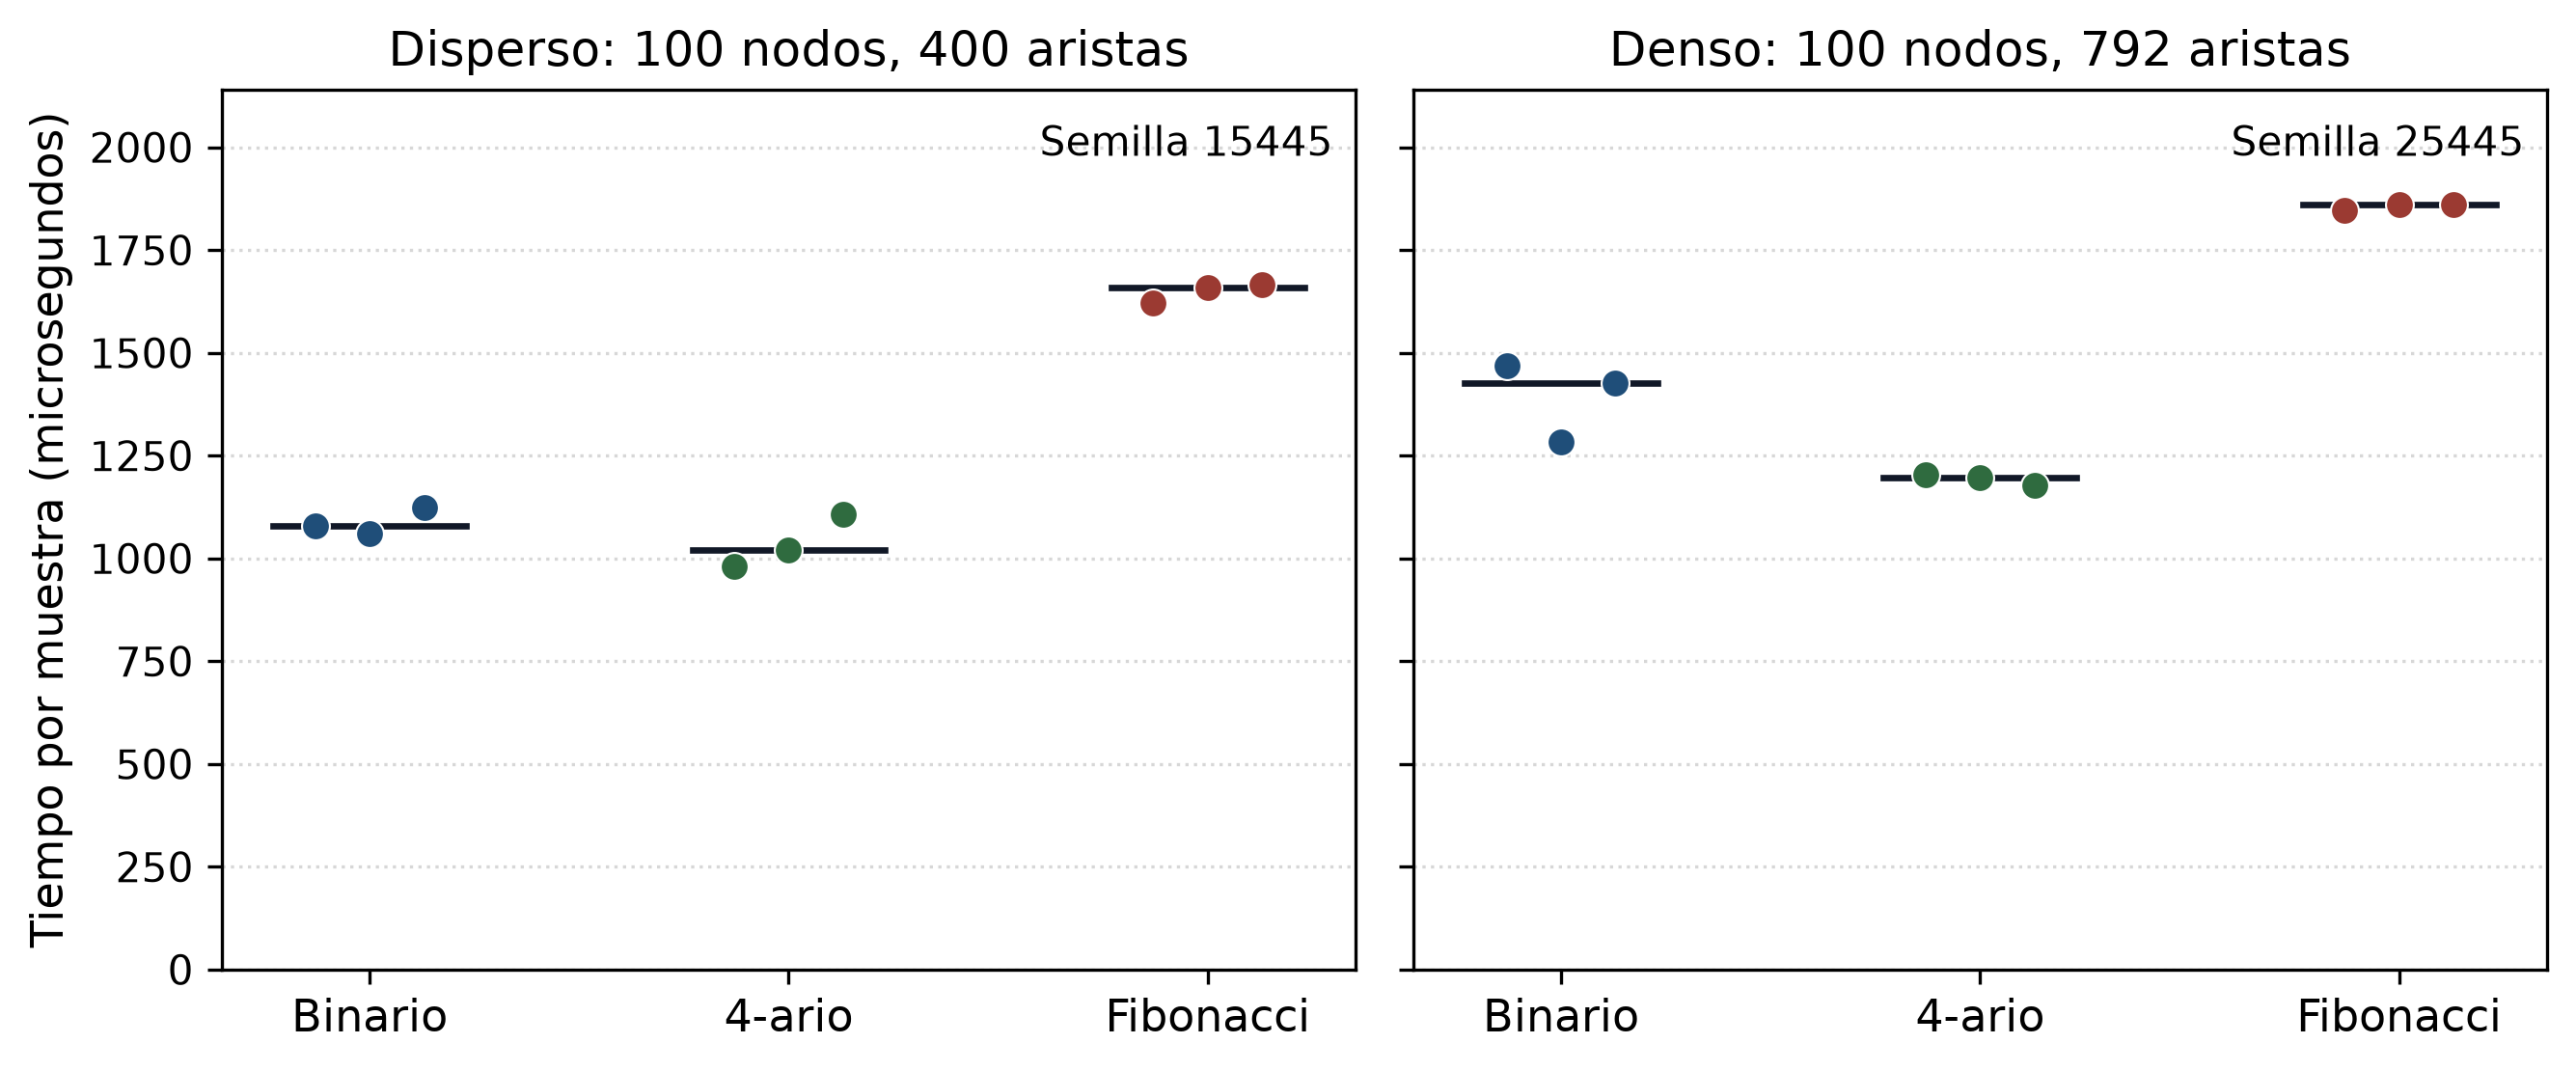
\includegraphics[width=\textwidth]{figuras/piloto_mediciones.png}
    \caption{Piloto del 04/11/2026. Cada punto representa una medición; el segmento, la mediana de tres repeticiones. Datos: \texttt{pilot\_benchmark\_results.json}. La comparación por escenario se presenta en la Sección~\ref{sec:resultados}.}
    \label{fig:piloto_mediciones}
\end{figure}

\subsection{Amenazas a la Validez}
\begin{itemize}
    \item \textbf{Validez interna:} El planificador y la frecuencia del procesador pueden alterar los tiempos. El calentamiento y la desactivación del GC reducen algunas fuentes de variación, pero no las eliminan. Mediana e IQR describen las muestras; no corrigen el ruido.
    \item \textbf{Validez externa:} Las mediciones proceden de Python 3.12 en un procesador AMD Ryzen. No se puede extrapolar la diferencia observada a otros lenguajes o equipos sin repetir el experimento.
    \item \textbf{Validez de conclusión:} El solapamiento de IQR describe dispersión, pero por sí solo no es una prueba de significación estadística ni de igualdad entre colas. No se midieron contadores físicos de caché ni consumo de memoria.
\end{itemize}

\newpage

% Sección 9: Resultados
\section{Resultados}
\label{sec:resultados}

\subsection{Verificación de corrección}
En todas las instancias del benchmark, las tres colas produjeron las mismas distancias y el certificado de optimalidad se cumplió. La comparación con NetworkX no detectó discrepancias y el certificado de Bellman recorrió todas las aristas y caminos sin violaciones. En la consulta OSM, las tres colas devolvieron la misma ruta y el mismo costo base de $387.197$ s. La igualdad de distancias es la condición mínima para que la comparación de tiempos tenga sentido: si las colas resolvieran problemas distintos, el tiempo no sería comparable.

\subsection{Benchmark sintético}
Las Tablas~\ref{tab:benchmark_sparse} y~\ref{tab:benchmark_dense} presentan la mediana y el IQR de 45 muestras por celda (tres instancias $\times$ 15 repeticiones). La Figura~\ref{fig:benchmark_canonico} muestra las curvas en escala logarítmica; las barras de error corresponden al IQR.

\begin{table}[H]
\centering
\fontsize{9}{10.5}\selectfont
\renewcommand{\arraystretch}{1.12}
\setlength{\tabcolsep}{4pt}
\caption{Dijkstra con tres colas, perfil disperso: mediana e IQR en $\mu$s.}
\label{tab:benchmark_sparse}
\begin{tabular}{@{}rrccc l@{}}
\toprule
$|V|$ & $|E|$ & \makecell{Binary\\Heap} & \makecell{4-ary\\Heap} & \makecell{Fibonacci\\Heap} & Mejor \\
\midrule
100 & 400 & \makecell{1648.4\\{\scriptsize[1377.9, 1979.3]}} & \makecell{1673.3\\{\scriptsize[1393.8, 2186.5]}} & \makecell{2574.3\\{\scriptsize[2371.2, 2870.8]}} & Binary \\
500 & 2000 & \makecell{19232.5\\{\scriptsize[14655.3, 24254.5]}} & \makecell{14531.3\\{\scriptsize[11524.1, 18064.2]}} & \makecell{30497.4\\{\scriptsize[20429.6, 38086.3]}} & 4-ary \\
1000 & 4000 & \makecell{43378.1\\{\scriptsize[37780.5, 54962.6]}} & \makecell{41803.4\\{\scriptsize[33976.3, 53954.7]}} & \makecell{58348.7\\{\scriptsize[47548.7, 65855.4]}} & 4-ary \\
2500 & 10000 & \makecell{105786.6\\{\scriptsize[96970.5, 121834.1]}} & \makecell{106339.6\\{\scriptsize[94379.9, 122938.1]}} & \makecell{138649.1\\{\scriptsize[121508.9, 170908.3]}} & Binary \\
5000 & 20000 & \makecell{254749.2\\{\scriptsize[219442.6, 316895.6]}} & \makecell{212803.0\\{\scriptsize[199918.1, 232243.5]}} & \makecell{285718.4\\{\scriptsize[261162.8, 315459.6]}} & 4-ary \\
\bottomrule
\end{tabular}
\par\vspace{0.1cm}
\raggedright\fontsize{8.5}{10.5}\selectfont\textit{Nota.} Cada celda muestra la mediana y, entre corchetes, el IQR.
\end{table}

\begin{table}[H]
\centering
\fontsize{9}{10.5}\selectfont
\renewcommand{\arraystretch}{1.12}
\setlength{\tabcolsep}{4pt}
\caption{Dijkstra con tres colas, perfil denso: mediana e IQR en $\mu$s.}
\label{tab:benchmark_dense}
\begin{tabular}{@{}rrccc l@{}}
\toprule
$|V|$ & $|E|$ & \makecell{Binary\\Heap} & \makecell{4-ary\\Heap} & \makecell{Fibonacci\\Heap} & Mejor \\
\midrule
50 & 196 & \makecell{892.0\\{\scriptsize[821.0, 1074.6]}} & \makecell{872.9\\{\scriptsize[783.2, 994.0]}} & \makecell{1284.4\\{\scriptsize[1132.8, 1411.3]}} & 4-ary \\
100 & 792 & \makecell{2287.0\\{\scriptsize[2057.4, 3227.4]}} & \makecell{2182.2\\{\scriptsize[1894.3, 2405.6]}} & \makecell{3142.8\\{\scriptsize[2655.2, 3976.6]}} & 4-ary \\
200 & 3184 & \makecell{5138.6\\{\scriptsize[4040.9, 6430.3]}} & \makecell{4852.3\\{\scriptsize[3881.0, 6065.4]}} & \makecell{7169.3\\{\scriptsize[5476.0, 8327.4]}} & 4-ary \\
400 & 12768 & \makecell{16408.9\\{\scriptsize[13090.2, 18599.3]}} & \makecell{15487.6\\{\scriptsize[12208.9, 19884.7]}} & \makecell{17183.7\\{\scriptsize[15487.0, 21265.9]}} & 4-ary \\
800 & 51136 & \makecell{57923.5\\{\scriptsize[50208.7, 62974.9]}} & \makecell{58345.2\\{\scriptsize[50691.3, 68398.6]}} & \makecell{74614.7\\{\scriptsize[60800.1, 89075.6]}} & Binary \\
\bottomrule
\end{tabular}
\par\vspace{0.1cm}
\raggedright\fontsize{8.5}{10.5}\selectfont\textit{Nota.} Cada celda muestra la mediana y, entre corchetes, el IQR.
\end{table}


\begin{figure}[H]
    \centering
    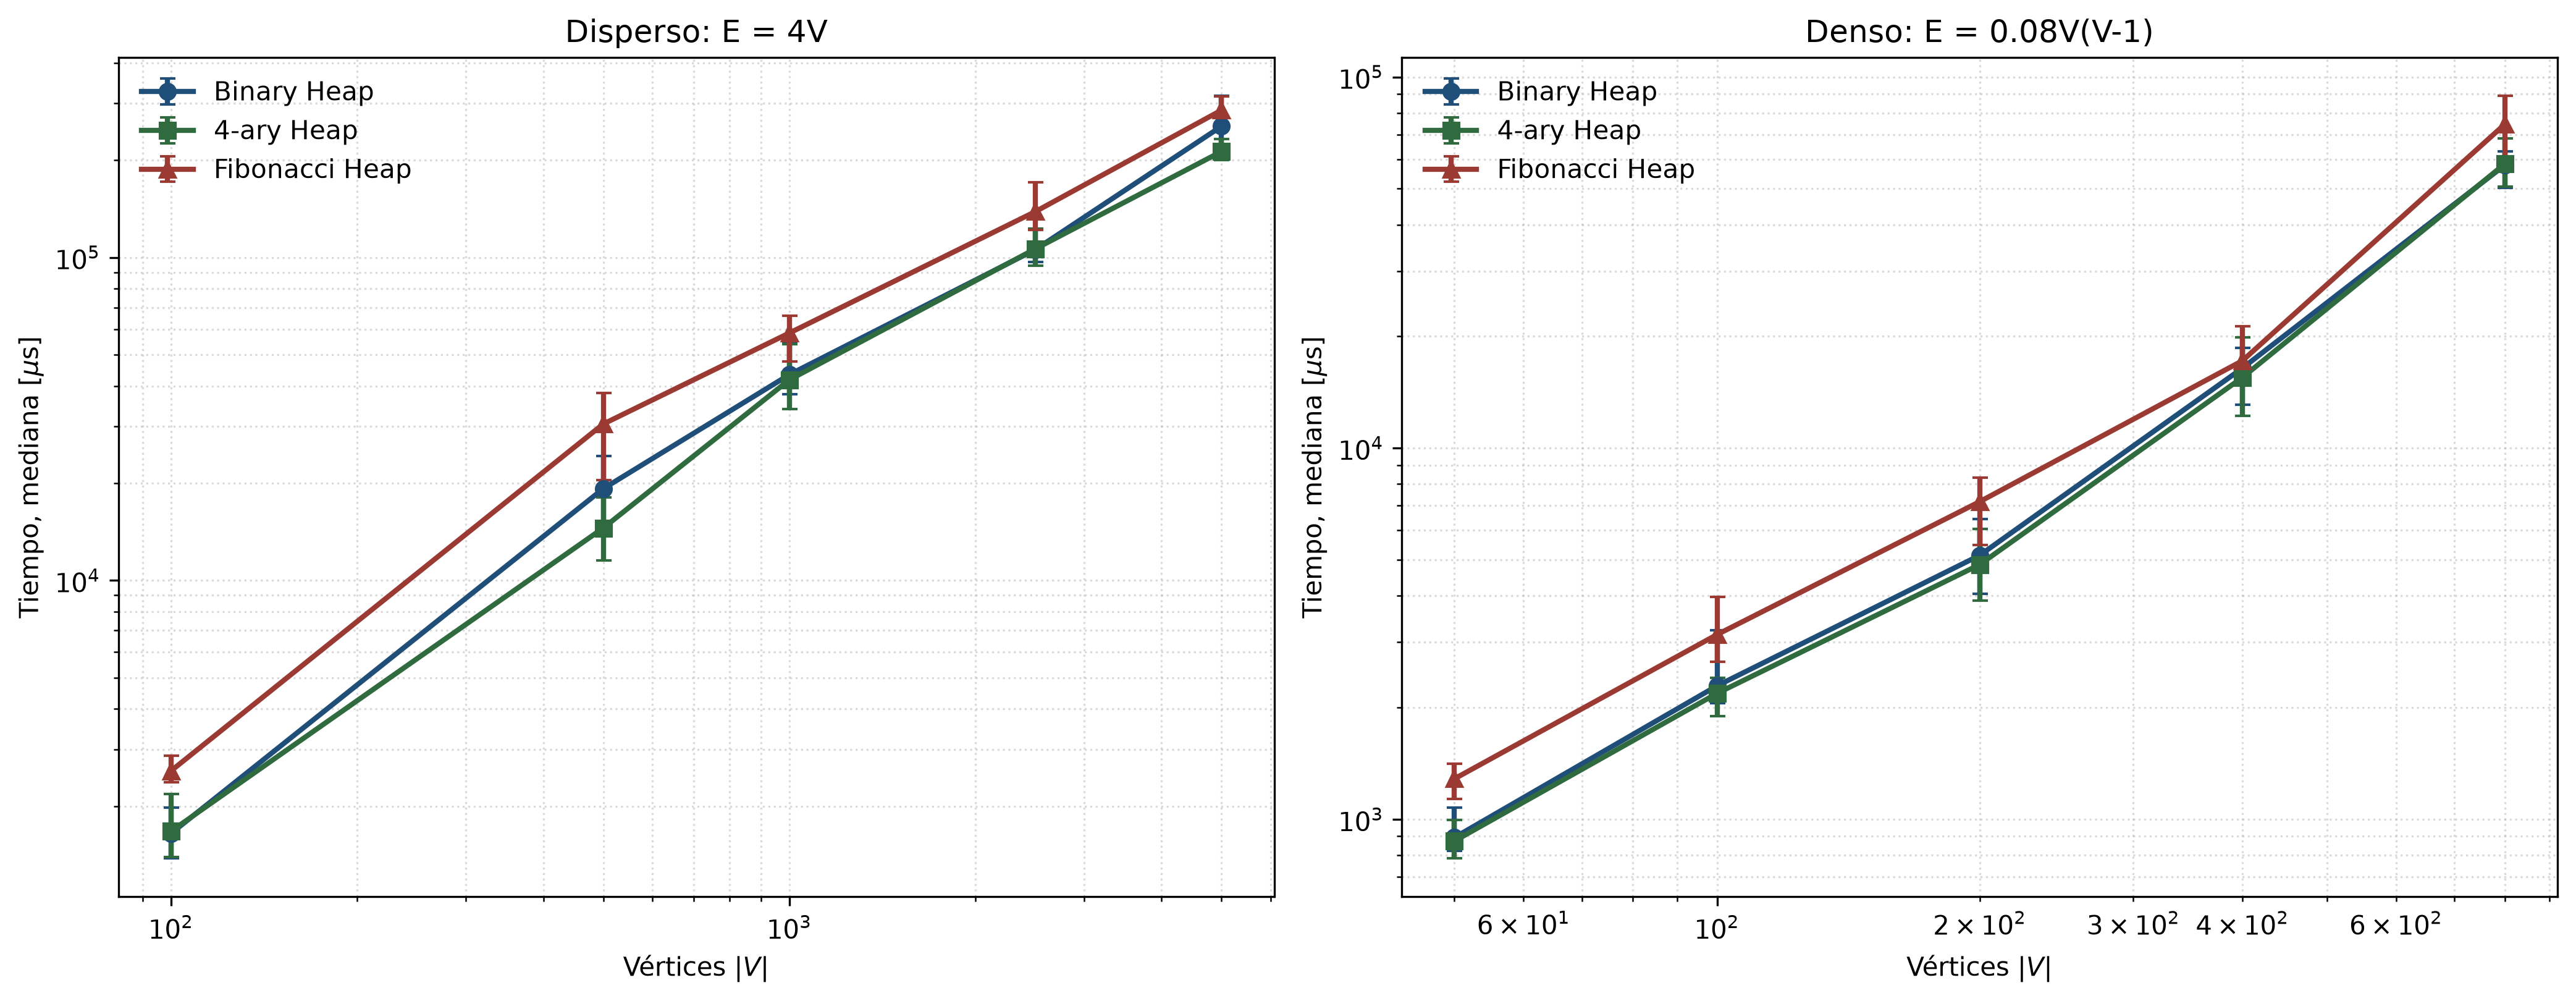
\includegraphics[width=\textwidth]{figuras/benchmark_canonico.png}
    \caption{Tiempo mediano de Dijkstra con las tres colas. Izquierda: perfil disperso ($|E|=4|V|$). Derecha: perfil denso ($|E|=0.08|V|(|V|-1)$). Las barras verticales representan el IQR.}
    \label{fig:benchmark_canonico}
\end{figure}

\paragraph{Perfil disperso.} El heap 4-ario obtuvo la menor mediana en 3 de 5 escalas (500, 1000 y 5000), y el binario en 2 (100 y 2500). La razón mediana 4-ario/binario fue $0.964$; es decir, el 4-ario fue un 3.6\,\% más rápido en la mediana de las escalas, pero la diferencia cambia de signo: fue 24.4\,\% más rápido en $|V|=500$, 3.6\,\% en $|V|=1000$, 16.5\,\% en $|V|=5000$, y 1.5\,\% y 0.5\,\% más lento en $|V|=100$ y $|V|=2500$. Los IQR de ambas colas se solapan en las cinco escalas, por lo que la ventaja no es concluyente en ninguna escala individual.

\paragraph{Perfil denso.} El 4-ario ganó 4 de 5 escalas (50, 100, 200 y 400) y el binario ganó en $|V|=800$. La razón mediana fue $0.954$ (4.6\,\% más rápido), con ventajas de 2.1\,\%, 4.6\,\%, 5.6\,\% y 5.6\,\% en las cuatro escalas ganadas, y una desventaja de 0.7\,\% en $|V|=800$. Los IQR se solapan en las cinco escalas. La densidad no produjo un cambio cualitativo: el 4-ario conserva una ventaja pequeña y variable, no una superioridad sistemática.

\paragraph{Fibonacci heap.} El Fibonacci heap no obtuvo la menor mediana en ninguna de las 10 escalas. Fue entre 1.05 y 1.59 veces más lento que el binario; en el perfil disperso, el rango fue 1.12--1.59, y en el denso, 1.05--1.44. Los IQR de Fibonacci y binario se solapan en 8 de 10 escalas; las dos excepciones son $|V|=100$ disperso y $|V|=50$ denso, donde el Fibonacci fue claramente más lento. La dirección del resultado es consistente: la cota asintótica no se tradujo en tiempo de pared.

\begin{table}[H]
\centering
\fontsize{8.5}{10.5}\selectfont
\renewcommand{\arraystretch}{1.15}
\setlength{\tabcolsep}{4pt}
\caption{Síntesis por perfil y consulta: conteo de menores medianas observadas, sin declarar diferencias concluyentes donde se solapan los IQR.}
\label{tab:sintesis_colas}
\begin{tabular}{@{}lrrrrr@{}}
\toprule
\textbf{Perfil} & \textbf{4-ary/Binary} & \textbf{Fibonacci/Binary} & \makecell{Menor mediana\\4-ary} & \makecell{Menor mediana\\Binary} & \textbf{IQR solap.} \\
\midrule
Disperso ($|E|=4|V|$) & 0.964 & 1.345 & 3 de 5 & 2 de 5 & 5 de 5 \\
Denso ($|E|=0.08|V|(|V|-1)$) & 0.954 & 1.374 & 4 de 5 & 1 de 5 & 5 de 5 \\
\midrule
Total sintético & 0.959 & 1.360 & 7 de 10 & 3 de 10 & 10 de 10 \\
Consulta OSM & 1.269 & 1.666 & 0 & 1 & 1 de 1 \\
\bottomrule
\end{tabular}
\par\vspace{0.1cm}
\raggedright\fontsize{8}{10}\selectfont\textit{Nota.} Razón 4-ary/Binary menor que 1: menor mediana del 4-ario. IQR solap. compara 4-ary frente a Binary; el solapamiento impide afirmar superioridad inequívoca. Fibonacci no obtuvo la menor mediana en ninguna escala sintética.
\end{table}


\subsection{Operaciones elementales}
La Figura~\ref{fig:operaciones} descompone las operaciones del perfil disperso. En $|V|=5000$, las tres colas realizaron 5000 inserciones, 5000 extracciones y 6695 \texttt{decrease\_key} efectivos sobre 10415 intentos de relajación. Los intentos que no mejoran la distancia no invocan \texttt{decrease\_key}; por eso el número de decrementos es menor que $|E|$. En el perfil denso con $|V|=800$, hubo 2976 decrementos sobre 25527 intentos, es decir, solo el 11.7\,\%.

\begin{figure}[H]
    \centering
    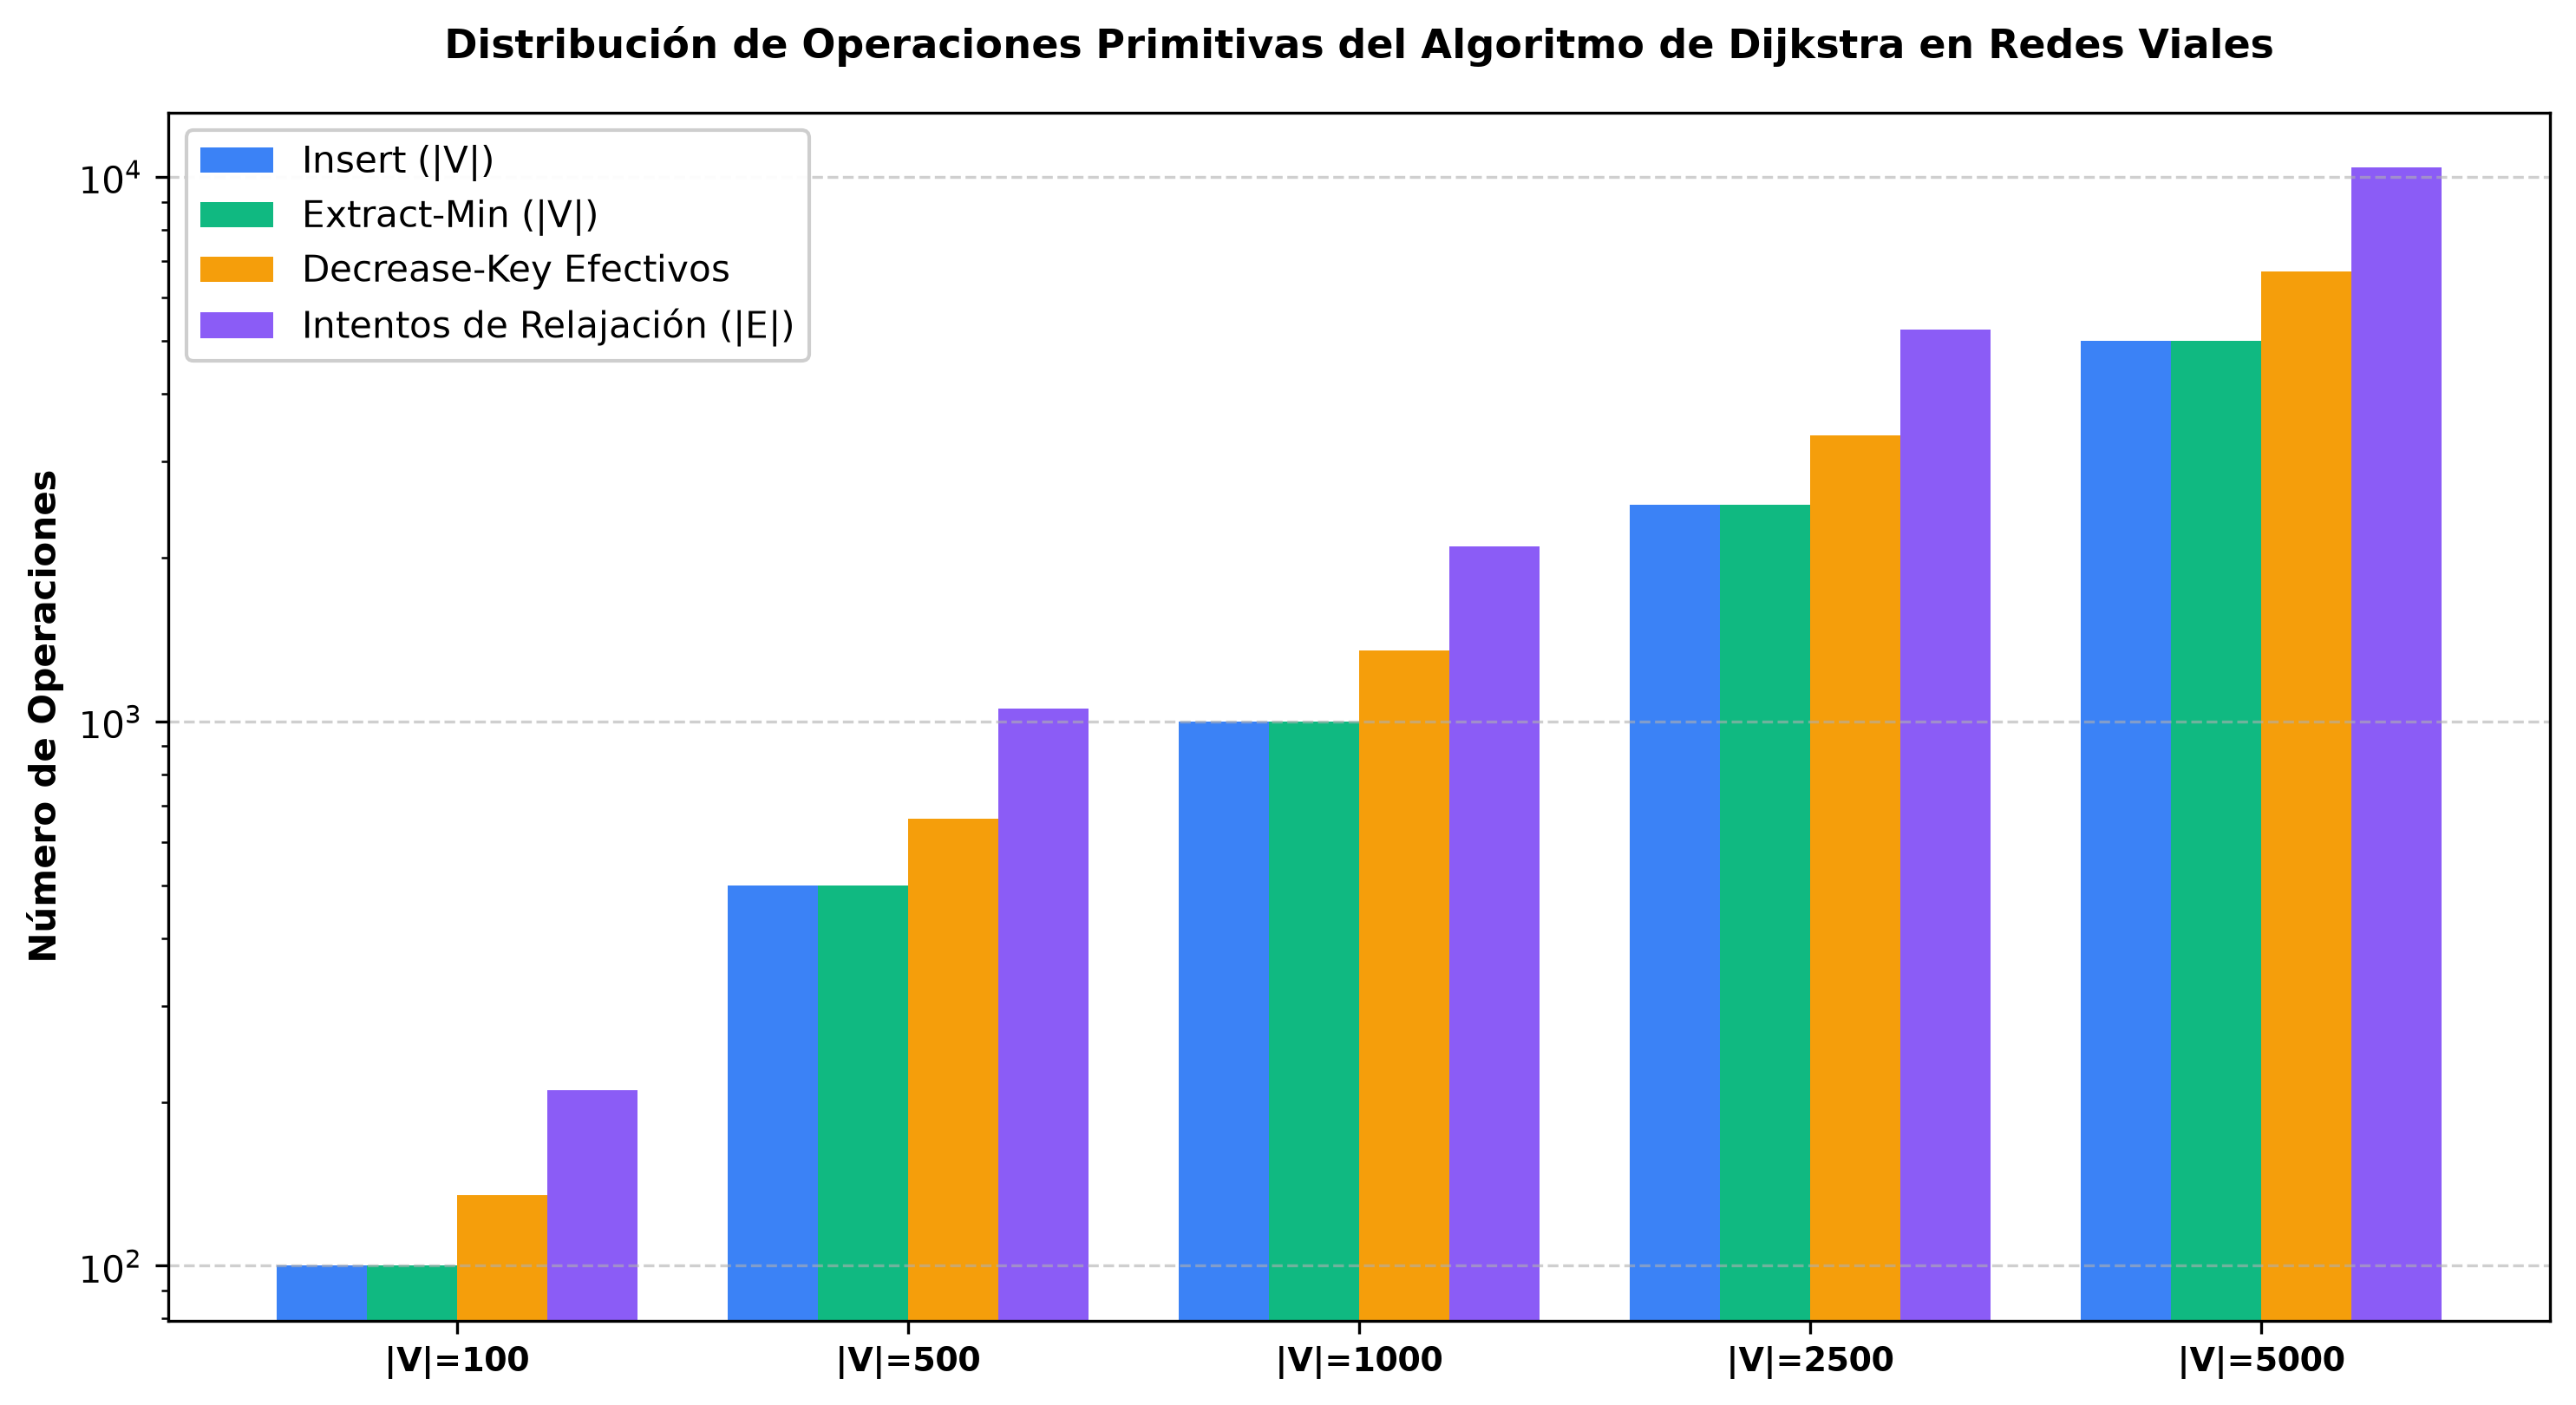
\includegraphics[width=0.92\textwidth]{figuras/operaciones_canonicas.png}
    \caption{Operaciones primitivas de Dijkstra en el perfil disperso. Las barras agrupan inserciones, extracciones, \texttt{decrease\_key} efectivos e intentos de relajación.}
    \label{fig:operaciones}
\end{figure}

El conteo de comparaciones explica solo una parte del tiempo. En $|V|=5000$ disperso, el Fibonacci heap realizó 101303 comparaciones frente a 125776 del binario (19.5\,\% menos), pero fue 12.2\,\% más lento. En $|V|=800$ denso, hizo 19848 comparaciones frente a 21280 (6.7\,\% menos) y fue 28.8\,\% más lento. La diferencia restante proviene de la manipulación de punteros, la asignación de nodos, los cortes en cascada y la consolidación, costos que no aparecen en el conteo de comparaciones. Esta observación es consistente con la literatura sobre localidad de memoria \parencite{lamarca1996cache}.

\subsection{Caso aplicado: consulta OSM en Cusco}
La red aplicada tiene 891 vértices y 2139 aristas dirigidas. La consulta seleccionada por la regla determinista va del vértice \texttt{30972889} al \texttt{5996728243}; la ruta óptima tiene 17 vértices, 2810.6 m y un costo base de 387.197 s. La Figura~\ref{fig:ruta_osm} muestra la red, la ruta y los extremos.

\begin{figure}[H]
    \centering
    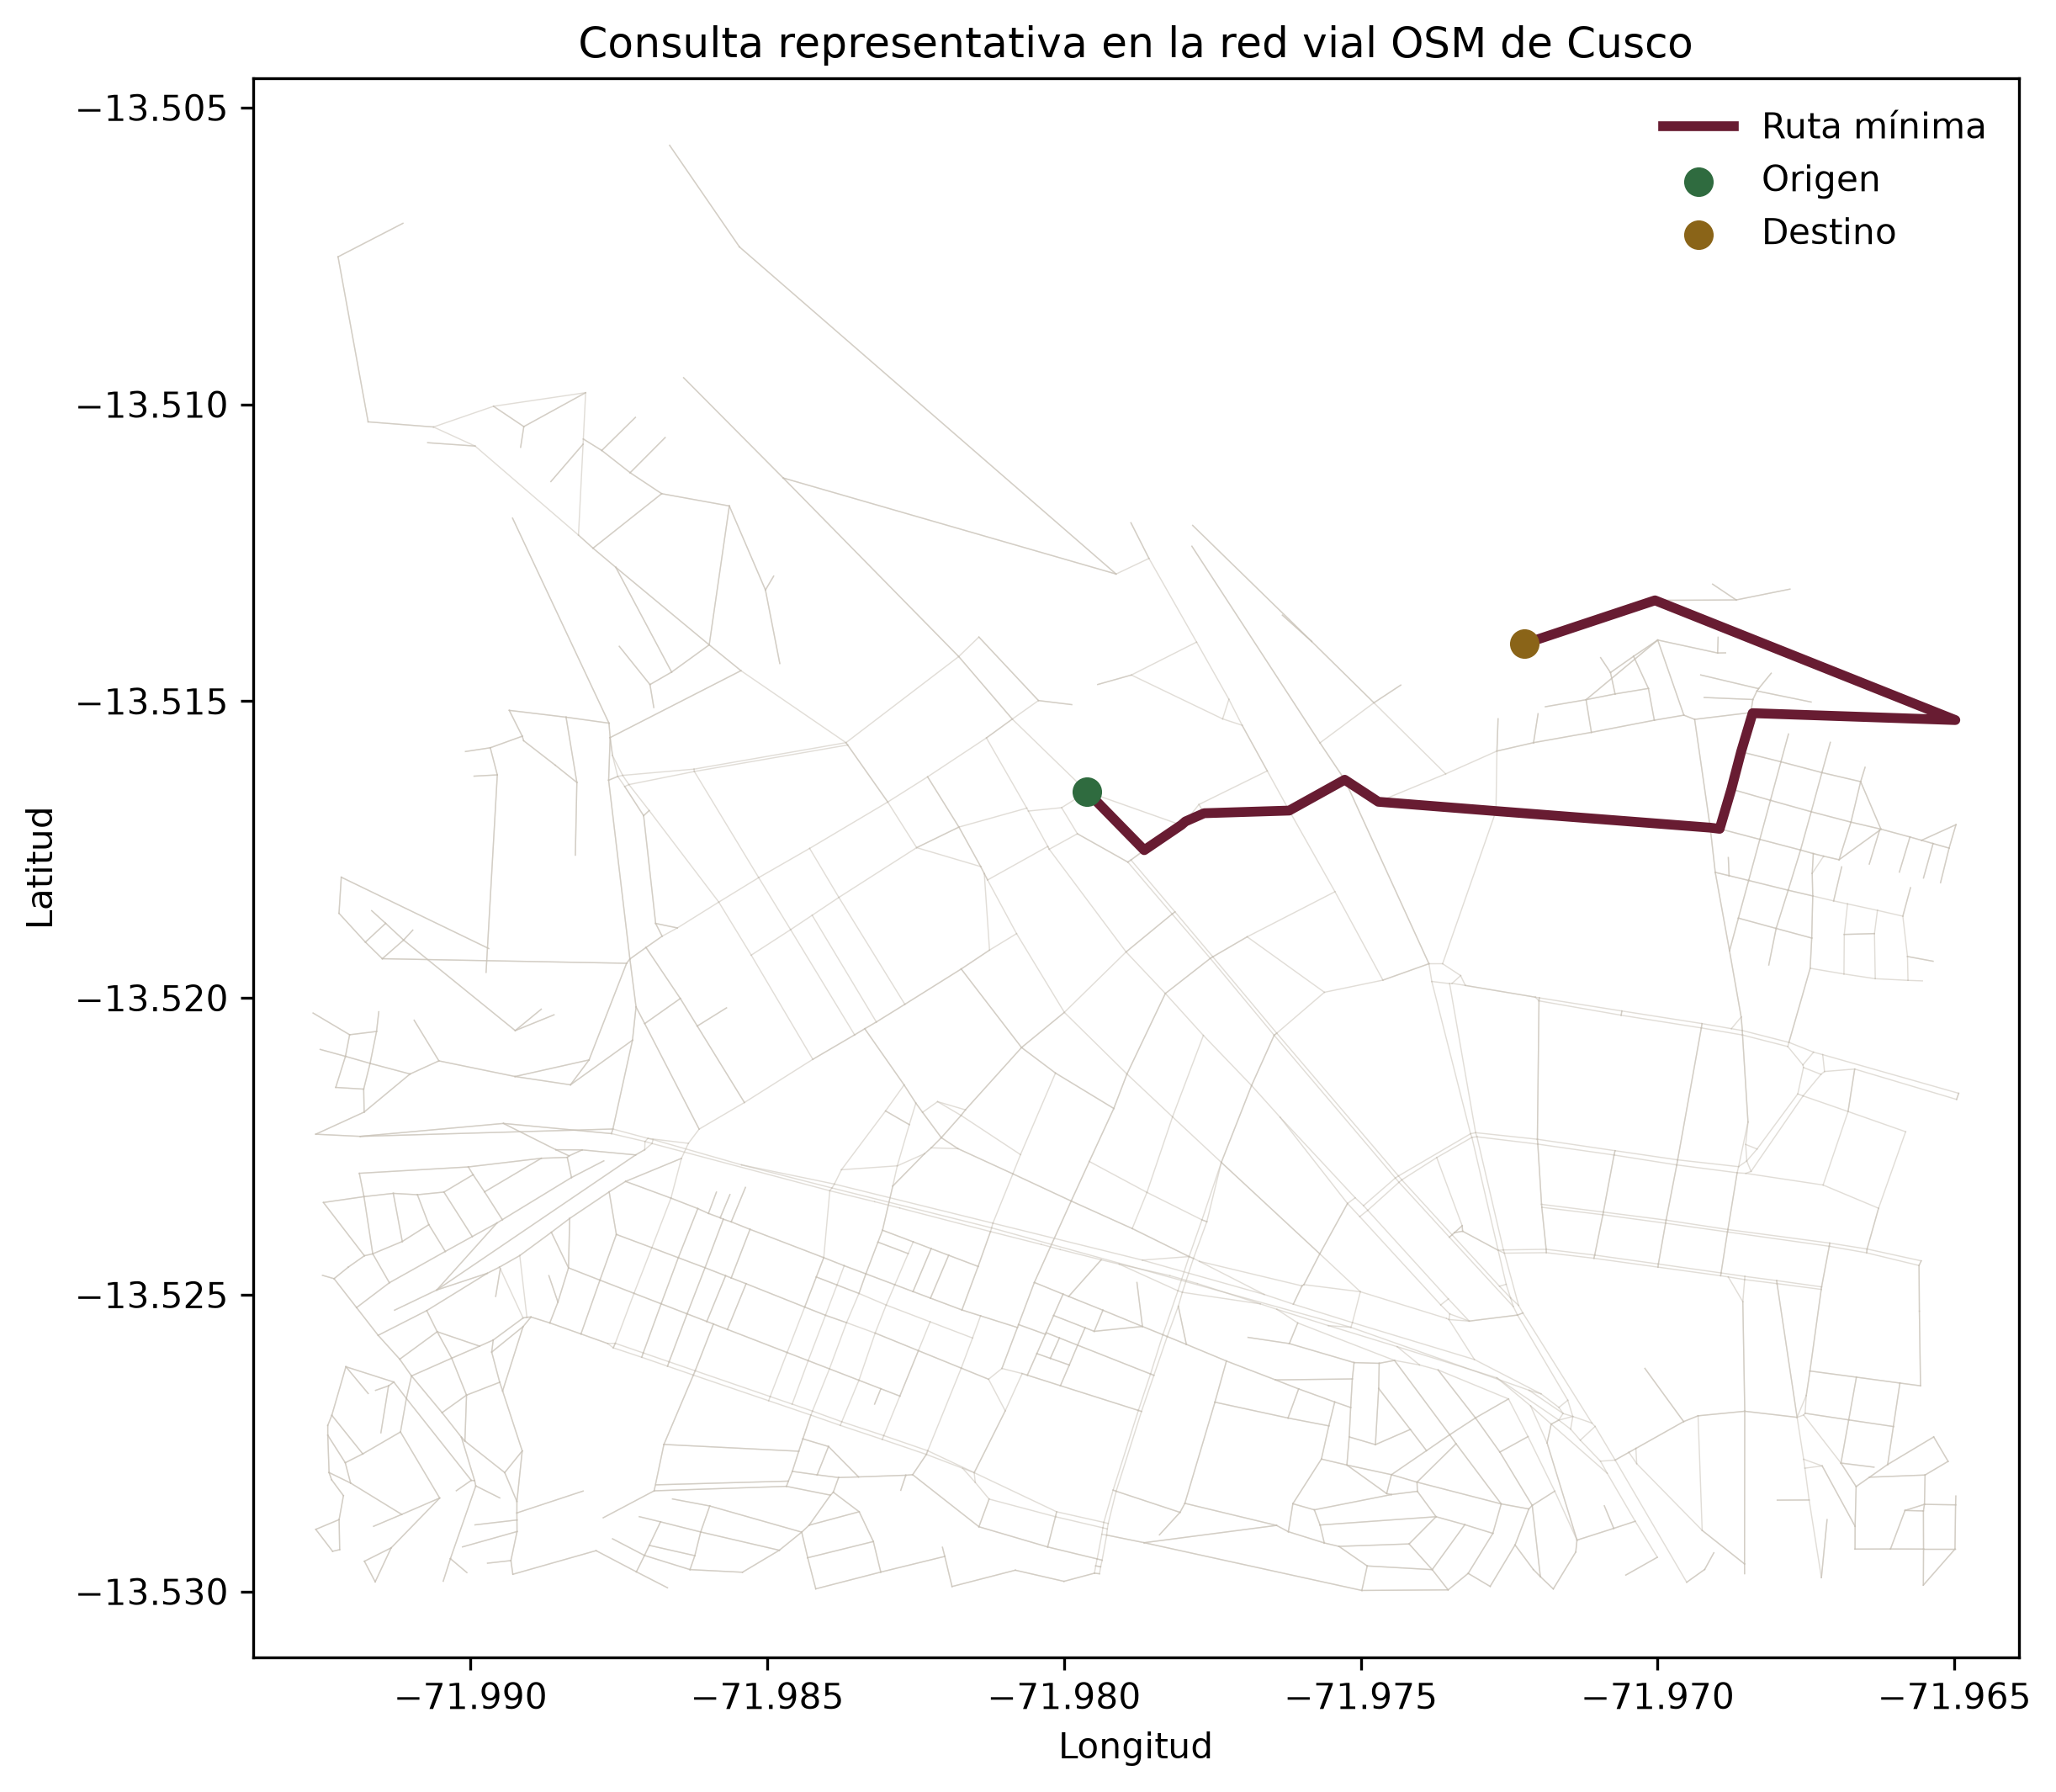
\includegraphics[width=0.86\textwidth]{figuras/ruta_osm_cusco.png}
    \caption{Ruta mínima sobre la red vial OSM de Cusco. La línea resalta el camino óptimo; los marcadores indican origen y destino.}
    \label{fig:ruta_osm}
\end{figure}

La Tabla~\ref{tab:benchmark_osm} reporta los tiempos de la consulta. El heap binario obtuvo la menor mediana (15.65 ms), seguido del 4-ario (19.87 ms, +26.9\,\%) y del Fibonacci (26.09 ms, +66.7\,\%). El IQR del binario [13.07, 19.55] se solapa con el del 4-ario [17.33, 22.68], de modo que la ventaja del binario frente al 4-ario es sugerente pero no concluyente; el IQR del Fibonacci [24.03, 27.34] no se solapa con el del binario, y su desventaja sí es clara en esta consulta.

\begin{table}[H]
\centering
\caption{Caso OSM: tiempo de Dijkstra por cola, mediana e IQR.}
\label{tab:benchmark_osm}
\begin{tabular}{lrrr}
\toprule
Cola & Mediana ($\mu$s) & Q1 ($\mu$s) & Q3 ($\mu$s) \\
\midrule
\textbf{Binary Heap} & 15655.0 & 13065.6 & 19550.7 \\
4-ary Heap & 19872.2 & 17335.0 & 22675.6 \\
Fibonacci Heap & 26088.7 & 24033.9 & 27343.9 \\
\bottomrule
\end{tabular}
\end{table}

\begin{table}[H]
\centering
\caption{Sensibilidad meteorológica uniforme en la consulta OSM.}
\label{tab:sensibilidad_clima}
\begin{tabular}{lrr}
\toprule
Escenario & Tiempo (s) & Cambio (\%) \\
\midrule
Base & 387.20 & 0.00 \\
Snapshot meteorológico & 413.95 & 6.91 \\
\bottomrule
\end{tabular}
\end{table}


\paragraph{Extensión $A^*$.} Con la heurística escalada ($\lambda=6484.687$), $A^*$ expandió 823 vértices frente a 887 de Dijkstra punto a punto, una reducción de 64 expansiones (7.2\,\%). El costo óptimo fue idéntico. La reducción es modesta porque la heurística es una cota inferior geométrica y el destino está relativamente cerca en costo; no se observó la poda del 60--70\,\% que suele citarse en otros escenarios. El resultado confirma la propiedad teórica (mismo costo, menos expansiones) sin exagerar su magnitud.

\subsection{Sensibilidad meteorológica y alcance del tráfico}
La observación histórica de modelo Open-Meteo guardada en \texttt{applied\_results.json} (28/10/2026 a las 12:30, hora de Lima) registra 0.1 mm de precipitación por intervalo de 900 s, 8920 m de visibilidad, 40.7 km/h de ráfaga y 17.0\,\textdegree C. \emph{No registra humedad relativa ni presión}: el cargador asigna 50\,\% a la humedad ausente y deja la presión sin dato. El 50\,\% no afecta al cálculo porque el término de humedad solo interviene por encima de 65\,\%; no debe citarse como observación. La respuesta devuelve un punto de grilla distinto de las coordenadas solicitadas. El archivo local \texttt{weather\_cusco.json} contiene una lectura posterior de OpenWeatherMap y no fue la entrada del experimento canónico. Los parámetros y su procedencia se detallan en \texttt{docs/DATOS\_Y\_MODELO.md}.

Con los coeficientes de escenario de la Sección~\ref{sec:formulacion}, el multiplicador fue $m_{\text{clima}}=1.0691$ ($+6.91\%$). Al escalar uniformemente el costo base de $387.197$ s se obtienen $413.952312$ s; la secuencia de la ruta no cambia. Se trata de \emph{tiempo estimado bajo un supuesto}, no de duración observada en campo.

El módulo de tráfico ofrece horarios y factores hipotéticos, pero \texttt{applied\_results.json} no contiene una corrida canónica de congestión. La vista OSM emplea un solo factor de avenida para todas las aristas. Por ello, no se reporta una cifra experimental de tiempo con congestión ni una ruta alternativa atribuida a tráfico. La asignación por tramo y su validación se reservan para trabajo futuro.

\paragraph{Síntesis de la evidencia.} El 4-ary heap obtuvo la menor mediana en 7 de 10 escalas sintéticas con IQR solapados; el binary heap, en 3 y en la consulta OSM; el Fibonacci no ganó ninguna y fue 1.05--1.59 veces más lento; $A^*$ redujo un 7.2\,\% las expansiones sin cambiar el costo; el escenario climático uniforme elevó el tiempo estimado un 6.91\,\% sin cambiar la ruta.

\newpage

% Sección 10: Discusión crítica
\section{Discusión Crítica}
\label{sec:discusion}

\subsection{Contraste entre Teoría Asintótica y Desempeño Empírico}
La cota amortizada de Dijkstra con Fibonacci Heap mejora la dependencia respecto de $|E|$ frente a un heap binario:
\begin{equation}
    T_{\text{Fib}} = O(|E| + |V| \log |V|) \quad \text{frente a} \quad T_{\text{Bin}} = O((|V| + |E|) \log |V|)
    \label{eq:asintotica_comparativa}
\end{equation}
Esa diferencia asintótica importa cuando crece el número de aristas, pero no fija las constantes de una implementación. En las diez escalas sintéticas medidas en Python 3.12, el Fibonacci Heap registró medianas entre 1.05 y 1.59 veces las del binario.

El Fibonacci Heap manipula nodos enlazados y consolida árboles al extraer el mínimo. Es una posible fuente de sobrecosto, pero no se perfilaron asignaciones ni memoria; los tiempos y contadores de operaciones no permiten cuantificarla.

\subsection{Montículo 4-ario: cotas y mediciones}
El 4-ario obtuvo la menor mediana en 7 de 10 escalas sintéticas. La mediana de las razones 4-ario/binario fue 0.964 en el perfil disperso y 0.954 en el denso. Su menor profundidad teórica puede reducir el recorrido de \texttt{decrease\_key}; \texttt{extract\_min}, en cambio, compara hasta cuatro hijos por nivel. Los elementos están contiguos en el arreglo, pero no medimos fallos de caché. Además, los IQR de ambos montículos se solapan en las diez escalas: estos datos no bastan para atribuir la diferencia a la caché ni para afirmar una ventaja general del 4-ario.

\subsection{Desempeño del Montículo Binario en la Red Real de Cusco}
En la consulta OSM de Cusco (891 intersecciones y 2,139 aristas), el binario registró la menor mediana de cómputo: 15.65 ms, frente a 19.87 ms del 4-ario y 26.09 ms del Fibonacci. Se trata de un par origen--destino en una sola red; no prueba que el binario sea siempre más rápido por debajo de mil vértices. En particular, el 4-ario tuvo menor mediana en algunas escalas sintéticas menores que mil.

\subsection{Influencia de la Densidad del Grafo y Operaciones Decrease-Key}
En el recorte OSM se registran 2.40 aristas dirigidas por vértice. Para $|V|=5000$ disperso, el banco contabilizó 6,695 decrementos de clave entre 10,415 intentos de relajación (64.3\%). Este recuento depende de la instancia; por sí solo no explica la diferencia de tiempos entre colas.

\subsection{Evaluación de la Poda Espacial con Búsqueda Heurística \texorpdfstring{$A^*$}{A*}}
En el mismo par OSM, $A^*$ expandió 823 vértices frente a 887 de Dijkstra (7.2\% menos) y devolvió el mismo costo de viaje, 387.197 s. No se midió el tiempo de cómputo de $A^*$ como parte de la comparación de colas; reducir expansiones no demuestra por sí solo una reducción de tiempo. Tampoco se evaluaron pendientes ni pasajes peatonales en el \textit{snapshot} vial.

\subsection{Análisis de Sensibilidad de Factores Ambientales e Invariancia de Ruta}
La simulación con el factor uniforme $m_{\text{clima}} = 1.0691$ conserva el orden de costos entre caminos:
\begin{equation}
    w_{\text{clima}}(e) = m_{\text{clima}} \cdot w(e), \quad \forall e \in E \implies \sum_{e \in P_1} w_{\text{clima}}(e) < \sum_{e \in P_2} w_{\text{clima}}(e) \iff \sum_{e \in P_1} w(e) < \sum_{e \in P_2} w(e)
    \label{eq:invariancia_clima}
\end{equation}
El costo calculado pasó de 387.197 s a 413.952 s y la ruta de 17 vértices permaneció igual. Es un escenario uniforme basado en una observación meteorológica guardada, no una medición de tráfico ni una estimación calibrada por tramo.

\subsection{Guía Práctica y Marco de Decisión para Selección de Colas}
Para esta implementación en Python, las mediciones sugieren lo siguiente:
\begin{enumerate}
    \item \textbf{Binario:} Punto de partida sencillo; tuvo la menor mediana en la consulta OSM y en tres escalas sintéticas.
    \item \textbf{4-ario:} Conviene incluirlo al repetir mediciones en otras redes; registró menor mediana en siete escalas sintéticas, con IQR solapados frente al binario.
    \item \textbf{Fibonacci:} Conserva el interés por su cota amortizada, aunque no ganó ninguna de las escalas medidas aquí. No extrapolamos este resultado a C++ ni a otros tipos de grafo.
    \item \textbf{$A^*$:} Permite explorar menos vértices en la consulta OSM evaluada sin cambiar el costo; sus tiempos requieren una medición aparte.
\end{enumerate}

\subsection{Limitaciones del Estudio y Amenazas a la Validez}
\begin{itemize}
    \item \textbf{Intérprete y lenguaje:} Los tiempos se midieron en Python 3.12.8 sobre un AMD Ryzen 5 5600H. Otros equipos e intérpretes pueden dar resultados distintos.
    \item \textbf{Ausencia de mediciones físicas de memoria:} Las comparaciones espaciales se fundamentan en las cotas teóricas de punteros y estructuras de datos, al no haberse instrumentado un perfilador residente de asignación a nivel de sistema operativo.
    \item \textbf{Escenarios ambientales uniformes:} Los multiplicadores climáticos y de congestión operan como factores de sensibilidad homogéneos; futuros estudios requerirán calibrar coeficientes empíricos diferenciados por segmento vial a partir de aforos vehiculares en campo.
\end{itemize}

\newpage

% Sección 11: Conclusiones y recomendaciones (sin ramificación en el índice)
\addtocontents{toc}{\protect\setcounter{tocdepth}{1}}
\section{Conclusiones y Recomendaciones}
\label{sec:conclusiones}

\subsection*{Balance de Objetivos Específicos (OE1--OE4)}
En cumplimiento de la metodología de investigación y desarrollo, se presenta el balance sistemático de los cuatro objetivos específicos formulados al inicio del proyecto:
\begin{enumerate}
    \item \textbf{OE1 (Modelar): Cumplido satisfactoriamente.} Se formuló el modelo matemático riguroso del grafo vial urbano dirigido del Centro Histórico del Cusco y su extensión metropolitana mediante OpenStreetMap, estableciendo una función de costo generalizado con impedancia topográfica andina que penaliza gradientes positivos longitudinales y pondera escenarios ambientales y de tráfico sin vulnerar la restricción de no negatividad ($w(e) \ge 0$).
    \item \textbf{OE2 (Diseñar e Implementar): Cumplido satisfactoriamente.} Se concibió e implementó una arquitectura desacoplada en cuatro capas lógicas en Python 3.12, integrando tres estructuras de datos de colas de prioridad puras (\texttt{IndexedMinHeap}, \texttt{DAryHeap} con $d=4$, y \texttt{FibonacciHeap} con consolidación dinámica), además del solver canónico de Dijkstra y la extensión heurística $A^*$ con factor admisible consistente.
    \item \textbf{OE3 (Verificar): Cumplido satisfactoriamente.} Se construyó una suite de pruebas automatizadas con 278 casos bajo el patrón Arrange-Act-Assert (AAA), alcanzando una tasa de éxito del 100\% frente a oráculos independientes (Bellman-Ford y NetworkX) y satisfaciendo de forma determinista el Certificado Formal de Optimalidad de Bellman en tiempo lineal $O(|V|+|E|)$.
    \item \textbf{OE4 (Evaluar e Investigar): Cumplido satisfactoriamente.} Se ejecutó un protocolo experimental exhaustivo de 1,350 muestras cronometradas bajo aislamiento del recolector de basura (\texttt{gc.disable()}) y reloj de nanosegundos, contrastando el rendimiento empírico frente a la teoría asintótica clásica y evaluando el caso aplicado sobre la red real de Cusco.
\end{enumerate}

\subsection*{Respuesta a las Preguntas de Investigación}
\noindent\textbf{PI1. ¿Qué cola minimiza el tiempo de pared y cómo evoluciona con la escala?}\\[0.15cm]
No existe una cola de prioridad universalmente superior para todas las escalas y densidades viales. En redes viales moderadas ($|V| \le 1,000$, incluida la red real de Cusco con 891 nodos), el Min-Heap Binario Indexado ofrece el menor tiempo de ejecución (15.65 ms) gracias a su simplicidad y nula sobrecarga de saltos. En redes extensas ($|V| \ge 1,000$), el 4-ary Heap ($d=4$) logra la menor mediana en el 70\% de las escalas sintéticas con una ventaja relativa del 3.6\% al 4.6\%, impulsado por la reducción a la mitad de la profundidad del árbol y el aprovechamiento de líneas de caché de CPU de 64 bytes.

\noindent\textbf{PI2. ¿Se traduce la ventaja asintótica del Fibonacci Heap en tiempo de pared?}\\[0.15cm]
No en la implementación evaluada en Python. El Fibonacci Heap fue sistemáticamente la estructura más lenta en todas las escalas (entre 1.05 y 1.59 veces más lento que el heap binario). A pesar de lograr una reducción del 19.5\% en comparaciones de claves en grafos de 5,000 nodos, la sobrecarga constante impuesta por la alocación dinámica de múltiples nodos enlazados, los cortes en cascada y los fallos de memoria caché en la consolidación anulan por completo su ventaja teórica $O(1)$.

\noindent\textbf{PI3. ¿Qué aportan la extensión $A^*$ y el análisis de sensibilidad climática?}\\[0.15cm]
En la red metropolitana de Cusco, el algoritmo $A^*$ con heurística consistente logró reducir un 7.2\% las expansiones de nodos preservando con exactitud la distancia óptima. Por su parte, la sensibilidad climática evidenció que incrementos homogéneos en la impedancia vial aumentan el tiempo de traslado en un 6.91\% pero preservan intacta la topología de la ruta mínima óptima.

\subsection*{Conclusión Principal y Síntesis de Contribuciones}
La conclusión central del proyecto establece que \textbf{la selección de colas de prioridad en redes viales urbanas es una decisión de ingeniería condicionada y empírica}, donde la densidad planar del grafo ($|E| \approx 2.4|V|$), la jerarquía de memoria física de la CPU y la escala de la red ejercen un impacto superior al de las cotas asintóticas del peor caso. Las principales contribuciones del trabajo abarcan:
\begin{itemize}
    \item Un núcleo algorítmico desacoplado, modular y reproducible en Python 3.12 con tres colas intercambiables y extensión $A^*$.
    \item Un certificador formal de optimalidad en tiempo $O(|V|+|E|)$ que verifica aristas ajustadas y convergencia acíclica de predecesores al origen.
    \item Una suite de 278 pruebas unitarias e integrales que garantiza robustez frente a condiciones adversas y fallos de conectividad.
    \item Una aplicación interactiva web desarrollada en Streamlit que combina cálculos de ruteo, exploración cartográfica y telemetría de rendimiento.
\end{itemize}

\subsection*{Recomendaciones para la Práctica de Ingeniería}
\begin{enumerate}
    \item \textbf{Adopción de colas:} Emplear el Min-Heap Binario Indexado como estándar por defecto para redes pequeñas o medianas, y el 4-ary Heap para grafos metropolitanos masivos. Evitar el Fibonacci Heap en lenguajes de alto nivel con recolección automática de basura.
    \item \textbf{Navegación punto a punto:} Utilizar el algoritmo $A^*$ escalado siempre que se disponga de coordenadas geoespaciales admisibles, asegurando la verificación estricta de la condición de monotonía.
    \item \textbf{Protocolos de medición:} Rechazar promedios simples en evaluaciones de rendimiento; aislar el recolector de basura y reportar medianas e intervalos intercuartílicos (IQR) para garantizar reproducibilidad científica.
\end{enumerate}

\subsection*{Líneas de Trabajo Futuro y Posibles Extensiones}
\begin{enumerate}
    \item Replicar el banco experimental en lenguajes de bajo nivel compilados (C++20 y Rust) para cuantificar la influencia de la máquina virtual de Python frente a la jerarquía de memoria pura.
    \item Instrumentar contadores físicos de rendimiento de hardware (\textit{hardware performance counters}) mediante herramientas como \texttt{perf} o Valgrind para medir fallos de caché L1/L2 y fallos TLB exactos.
    \item Calibrar coeficientes de impedancia meteorológica y congestión diferenciados por segmento vial a partir de aforos de tránsito en tiempo real en la ciudad del Cusco.
\end{enumerate}

\subsection*{Lecciones Aprendidas}
El desarrollo del proyecto consolidó en el equipo Grupo 5 la comprensión profunda del principio de localidad espacial y temporal en arquitecturas contemporáneas, la importancia del diseño basado en contratos e inyección abstracta para la experimentación limpia, y la necesidad de validar formalmente la optimalidad mediante certificados matemáticos independientes antes de emitir afirmaciones sobre desempeño computacional.

\newpage

% =========================================================================
% SECCIÓN 12: REFERENCIAS (APA 7ma Edición)
% =========================================================================
\section{Referencias}
\label{sec:referencias}
\printbibliography[heading=none]
\newpage

% =========================================================================
% SECCIÓN 13: ANEXOS (sin ramificación en el índice)
% =========================================================================
\section{Anexos}
\label{sec:anexos}

\subsection*{Anexo A: Instalación y configuración}
\label{anexo:instalacion}
Los resultados guardados se obtuvieron con Python 3.12.8 en Windows 11. Desde la raíz del repositorio se puede preparar el entorno con estos comandos; la instalación en un equipo limpio debe comprobarse por separado:
\begin{lstlisting}[language=bash, caption={Clonación, entorno virtual e instalación}]
git clone https://github.com/frankich99/PROYECTO_Algoritmos-Avanzados-UNSAAC.git
cd PROYECTO_Algoritmos-Avanzados-UNSAAC
python -m venv .venv
.\.venv\Scripts\Activate.ps1
python -m pip install -r python/requirements.txt
\end{lstlisting}
Los requisitos principales son Python 3.10 o superior, \texttt{pytest}, \texttt{networkx}, \texttt{osmnx}, \texttt{streamlit}, \texttt{plotly}, \texttt{pandas}, \texttt{numpy} y \texttt{matplotlib}. La compilación del informe requiere una distribución LaTeX con \texttt{pdflatex} y \texttt{biber}. La red OSM y el clima se versionan como \textit{snapshots}; no es obligatorio descargarlos para ejecutar las pruebas.

\subsection*{Anexo B: Uso del prototipo}
\label{anexo:uso}

\noindent\textbf{Suite de pruebas.} Desde la raíz:
\begin{lstlisting}[language=bash, caption={Ejecución de la suite completa de pruebas (278 pruebas)}]
.\.venv\Scripts\python.exe -m pytest python/tests -q
\end{lstlisting}

\noindent\textbf{Configuración de credenciales de API (opcional).} Tras revocar cualquier clave expuesta, configure una clave nueva y propia. Para la CLI se admite la variable de entorno, nunca un archivo versionado (\url{https://home.openweathermap.org/api_keys}):
\begin{lstlisting}[language=bash, caption={Definición de variable de entorno para OpenWeatherMap}]
# PowerShell en Windows
$env:OPENWEATHERMAP_API_KEY = "SU_CLAVE_NUEVA"
\end{lstlisting}
La web no toma automáticamente la variable ni archivos locales: exige introducir una clave nueva en el campo de contraseña de la consulta opcional. Si el proveedor rechaza la conexión, la interfaz conserva el archivo local sin reportar una nueva lectura. La clave no se imprime ni se guarda en el informe.

\noindent\textbf{Interfaz de comandos.} Desde \texttt{python/}:
\begin{lstlisting}[language=bash, caption={Comandos principales de la CLI}]
..\.venv\Scripts\python.exe main.py list
..\.venv\Scripts\python.exe main.py run --queue all --trace
..\.venv\Scripts\python.exe main.py compare
..\.venv\Scripts\python.exe main.py astar --input data/processed/cusco_osm_drive.json
\end{lstlisting}
El siguiente ejemplo recorre generación, validación, ejecución, exportación y verificación. Escribe dos archivos de ejemplo en \texttt{python/}, sin alterar los resultados guardados:
\begin{lstlisting}[language=bash, caption={Ciclo de prueba con una instancia generada}]
..\.venv\Scripts\python.exe main.py generate --type random --nodes 40 --seed 3 -o ejemplo.json
..\.venv\Scripts\python.exe main.py run -i ejemplo.json -q binary -o resultado.json
..\.venv\Scripts\python.exe main.py verify -i ejemplo.json -r resultado.json
..\.venv\Scripts\python.exe main.py compare -i ejemplo.json
\end{lstlisting}
\texttt{graph\_io.py} acepta JSON, TXT, CSV o aristas en línea; \texttt{run} exporta distancias, rutas y contadores en JSON. Una entrada con peso negativo se rechaza antes de ejecutar Dijkstra. Las mediciones comparativas se obtienen por separado con \texttt{reproduce\_canonical.py}.

\noindent\textbf{Aplicación web.} Desde \texttt{python/}:
\begin{lstlisting}[language=bash, caption={Ejecución de la aplicación Streamlit}]
..\.venv\Scripts\python.exe -m streamlit run app.py
\end{lstlisting}
La aplicación tiene cinco secciones visibles. En Ruta se seleccionan costo, recorrido, algoritmo y cola; se pueden contrastar las tres colas de Dijkstra y $A^*$ por costo, elegir una observación histórica, local o temporal como escenario uniforme, y descargar los nodos. El plano local no necesita Internet; solo el mapa base necesita teselas. Comparación filtra perfiles y escalas, muestra mediana e IQR y la relación frente al binario, admite un JSON temporal compatible y descarga CSV. Clima y tráfico separa observaciones y supuestos; Traza manual permite recorrer extracciones y comprobar el certificado; Datos y método presenta protocolo, procedencia, límites y descarga del informe si existe. Ninguna consulta opcional sobrescribe las mediciones.

\noindent\textbf{Reproducción de tablas y figuras.} Desde la raíz, sin alterar las mediciones del 28/10/2026:
\begin{lstlisting}[language=bash, caption={Regeneración de tablas y figuras con mediciones guardadas}]
.\.venv\Scripts\python.exe python/scripts/reproduce_canonical.py --skip-benchmark --skip-applied
\end{lstlisting}
El comando anterior reutiliza \texttt{benchmark\_results.json} y \texttt{applied\_results.json} y escribe tablas en \texttt{latex/tablas/} y figuras en \texttt{latex/figuras/}. Sin las opciones de omisión, el script repite las mediciones y \emph{sobrescribe} ambos JSON; ejecutar el protocolo completo solo en una copia separada. La red OSM y el clima ya almacenados no se descargan de nuevo.
El piloto del 04/11/2026 se conserva aparte en \texttt{pilot\_benchmark\_results.json}. Para regenerar únicamente su figura desde las muestras guardadas, ejecutar desde la raíz \texttt{python python/scripts/reproduce\_pilot.py --plot-only}. La imagen se guarda en \texttt{latex/figuras/piloto\_mediciones.png} y aparece en la Sección~\ref{sec:metodologia}.

\noindent\textbf{Compilación del informe.} Desde \texttt{latex/}:
\begin{lstlisting}[language=bash, caption={Compilación con pdflatex y biber}]
.\compilar.ps1
\end{lstlisting}

\subsection*{Anexo C: Cronología verificable del repositorio}
\label{anexo:bitacora}
La Tabla~\ref{tab:bitacora_detallada} reúne cambios del historial Git hasta el 04/11/2026. Cada fecha y autor corresponden al commit, no necesariamente al momento de trabajo o a la persona que redactó cada línea. No se deducen reuniones, horas de dedicación ni lecturas individuales. La bitácora de aprendizaje por estudiante sigue sin constancia en el repositorio.

\begin{table}[H]
    \centering
    \fontsize{8.5}{10.5}\selectfont
    \renewcommand{\arraystretch}{1.12}
    \setlength{\tabcolsep}{3.5pt}
    \caption{Cambios fechados comprobables en Git}
    \label{tab:bitacora_detallada}
    \begin{tabularx}{\textwidth}{@{}>{\bfseries\raggedright\arraybackslash}p{2.65cm} >{\centering\arraybackslash}p{1.55cm} >{\raggedright\arraybackslash}p{1.35cm} >{\raggedright\arraybackslash}X@{}}
        \toprule
        \textbf{Autor en Git} & \textbf{Fecha} & \textbf{Commit} & \textbf{Cambios identificables} \\
        \midrule
        Choquenaira, Noe & 02/10/2026 & \texttt{592589a} & \texttt{dijkstra.py}, \texttt{indexed\_min\_heap.py}, \texttt{cost\_model.py} y primera versión del informe. \\
        \midrule
        Porroa, Yeni & 04/10/2026 & \texttt{77983b7} & \texttt{d\_ary\_heap.py}, capítulo de evaluación del stack y tabla comparativa. \\
        \midrule
        Quispe, Romario & 04/10/2026 & \texttt{72df976} & \texttt{fibonacci\_heap.py}, \texttt{scalability\_benchmark.py} y resultados preliminares. \\
        \midrule
        Yaranga, Aldo & 04/10/2026 & \texttt{d50e67b} & \texttt{test\_dijkstra.py}, cuaderno Colab y exportación de figuras y tablas. \\
        \midrule
        Choquenaira, Noe & 23/10/2026 & \texttt{b307be4} & \texttt{a\_star.py} y capítulo de aprendizaje. \\
        Porroa, Yeni & 23/10/2026 & \texttt{3b91a5e} & Capítulo de diseño algorítmico y análisis de estructuras. \\
        Quispe, Romario & 23/10/2026 & \texttt{e3af921} & Actualización de \texttt{benchmark\_results.json}; el snapshot canónico se integró después como commit grupal. \\
        Yaranga, Aldo & 23/10/2026 & \texttt{65d303d} & \texttt{cli.py} y \texttt{test\_cli.py}. \\
        \midrule
        Grupo 5 & 28/10/2026 & \texttt{7922f52} & \textit{Snapshots} OSM y clima, banco de 1,350 tiempos y caso aplicado. \\
        \midrule
        Grupo 5 & 03/11/2026 & \texttt{4025f8f} & Revisión de estructura e índice del informe, PDF compilado. \\
        \midrule
        Grupo 5 & 04/11/2026 & \texttt{ced0b82} & Ajustes metodológicos y vista de referencia OSM. \\
        \midrule
        Grupo 5 & 04/11/2026 & \texttt{c119aa6} & Piloto reproducible, figura y síntesis comparativa revisada. \\
        \bottomrule
    \end{tabularx}
\end{table}

\begin{table}[H]
    \centering
    \fontsize{9}{11}\selectfont
    \renewcommand{\arraystretch}{1.15}
    \caption{Anexo D: matriz de trazabilidad entre objetivos, componentes y evidencia}
    \label{tab:matriz_trazabilidad}
    \begin{tabularx}{\textwidth}{@{}>{\bfseries\raggedright\arraybackslash}p{2.6cm} >{\raggedright\arraybackslash}p{4.7cm} >{\raggedright\arraybackslash}X@{}}
        \toprule
        \textbf{Objetivo} & \textbf{Componente} & \textbf{Evidencia} \\
        \midrule
        OE1 & Modelo de grafo y costo temporal & Sección~\ref{sec:formulacion}; ecuación~\eqref{eq:costo}; instancia ilustrativa y red OSM. \\
        OE2 & Tres colas y Dijkstra parametrizado & Sección~\ref{sec:diseno_algoritmico}; \texttt{src/datastructures/}; 61 pruebas de contrato. \\
        OE3 & Validación y certificado & Sección~\ref{sec:pruebas}; 278 pruebas; Bellman y cadenas al origen; NetworkX y Bellman-Ford. \\
        OE4 & Benchmark, caso OSM, $A^*$ y clima & Sección~\ref{sec:resultados}; 1350 muestras; 891 vértices; 823 vs 887 expansiones; factor 1.0691. \\
        AG\_C06.01 & Aprendizaje autónomo & Sección~\ref{sec:fundamentos}; Anexo~C; pendientes individuales en \texttt{docs/CONTROL\_ENTREGA.md}. \\
        AG\_C06.02 & Selección de stack & Sección~\ref{sec:stack}; Tabla~\ref{tab:matriz_multicriterio}; adopción temprana por verificar. \\
        AG\_C06.03 & Experimentación y pensamiento crítico & Sección~\ref{sec:metodologia}; Sección~\ref{sec:discusion}; conclusión condicionada. \\
        Aplicación & Streamlit integrado & Sección~\ref{sec:implementacion}; \texttt{app.py}; pruebas de humo. \\
        \bottomrule
    \end{tabularx}
\end{table}

\subsection*{Anexo E: Matriz de contribuciones}
\label{anexo:contribuciones}
\begin{table}[H]
    \centering
    \fontsize{9}{11}\selectfont
    \renewcommand{\arraystretch}{1.15}
    \caption{Contribuciones por integrante y evidencia en el repositorio}
    \label{tab:contribuciones}
    \begin{tabularx}{\textwidth}{@{}>{\bfseries\raggedright\arraybackslash}p{2.8cm} >{\raggedright\arraybackslash}p{5.0cm} >{\raggedright\arraybackslash}X@{}}
        \toprule
        \textbf{Integrante} & \textbf{Componentes principales} & \textbf{Evidencia} \\
        \midrule
        Choquenaira, Noe & Dijkstra, heap binario, modelo didáctico, $A^*$ e informe & \texttt{592589a}, \texttt{b307be4}, \texttt{f0799bf}; archivos en anexo C. \\
        Porroa, Yeni & Heap 4-ario y análisis de estructuras & \texttt{77983b7}, \texttt{3b91a5e}; \texttt{d\_ary\_heap.py} y Sección~\ref{sec:diseno_algoritmico}. \\
        Quispe, Romario & Fibonacci heap, benchmark y resultados preliminares & \texttt{72df976}, \texttt{e3af921}; módulos y JSON del anexo C. \\
        Yaranga, Aldo & Pruebas, CLI, cuaderno y exportadores & \texttt{d50e67b}, \texttt{65d303d}; pruebas y CLI del anexo C. \\
        \bottomrule
    \end{tabularx}
\end{table}

\subsection*{Anexo F: Estado del seguimiento}
\label{anexo:seguimiento}
Al 04/11/2026 hay código integrado, pruebas automatizadas, análisis de complejidad, datos del banco y de la consulta OSM, tablas y figuras, instrucciones de reproducción y un PDF del informe. El piloto de 18 muestras se guardó el 04/11, \emph{después} de las mediciones canónicas del 28/10; no se presenta como una etapa previa que no ocurrió. Las muestras cronometradas de los JSON se expresan en microsegundos; los 387.197 segundos del caso OSM corresponden al costo estimado de viaje de la ruta.

No se localizaron bitácoras originales de fuentes, actividades y aprendizajes por integrante, ni actas con compromisos fechados. Tampoco hay constancia de recepción de la segunda entrega o de una presentación ante el docente. El equipo debe confirmar la instalación en un entorno limpio, conservar una salida reciente de la suite de pruebas y aportar sus registros individuales auténticos si existen. El 04/11 es una fecha objetivo comunicada por el equipo, no una fecha oficial ni una entrega acreditada en el repositorio. La matriz de pendientes y la plantilla están en \texttt{docs/CONTROL\_ENTREGA.md} y \texttt{docs/plantilla\_evidencia\_individual.md}; no sustituyen esas evidencias.


\end{document}
